% LaTEX source code
% Last modified November 1st, 2005
% Steve Miller
% note that the percent sign comments out the rest of the line
% first, we set a document class. often use 12pt characters, though
% sometimes people do 11 or 10. you can do report or article, both similar
%\documentclass[12pt,letterpaper]{article}
\documentclass[12pt,reqno]{amsart}
\linespread{1}
\addtolength{\textwidth}{2cm} \addtolength{\hoffset}{-1cm}
\addtolength{\marginparwidth}{-1cm} \addtolength{\textheight}{2cm}
\addtolength{\voffset}{-1cm}
% below are some packages that are needed for certain symbols, graphics, colors.
% safest to just include these.
\usepackage{times}
\usepackage[T1]{fontenc}
\usepackage{mathrsfs}
\usepackage{latexsym}
\usepackage[dvips]{graphics}
\usepackage{epsfig}
\usepackage{hyperref, amsmath, amsthm, amsfonts, amscd, flafter,epsf}
\usepackage{amsmath,amsfonts,amsthm,amssymb,amscd}
\input amssym.def
\input amssym.tex
\usepackage{color}
\usepackage{enumerate}
\usepackage{hyperref}
\usepackage{url}
\usepackage{floatrow}
\usepackage{caption}
\usepackage{subcaption}
\usepackage{capt-of}
\usepackage{physics}
\newcommand{\todo}[1]{\textcolor{red}{\textbf{(#1)}}}

    %=======================================================

    %   THIS IS WHERE YOU PUT SHORTCUT DEFINITIONS

    %========================================================

% Note that we use a percent sign to comment out a line

% below are shortcut commands

%%%%%%%%%%%%%%%%%%%%%%%%%%%%%%%%%%%%%%%%%%%%%%%

% below are shortcuts for equation, eqnarray,

% itemize and enumerate environments

\newcommand\be{\begin{equation}}
\newcommand\ee{\end{equation}}
\newcommand\bea{\begin{eqnarray}}
\newcommand\eea{\end{eqnarray}}
\newcommand\bi{\begin{itemize}}
\newcommand\ei{\end{itemize}}
\newcommand\ben{\begin{enumerate}}
\newcommand\een{\end{enumerate}}
\newcommand{\ncr}[2]{\left({#1 \atop #2}\right)}
%%%%%%%%%%%%%%%%%%%%%%%%%%%%%%%%%%%%%%%%%%%%%%%%

% Theorem / Lemmas et cetera

\newtheorem{thm}{Theorem}[section]
\newtheorem{conj}[thm]{Conjecture}
\newtheorem{cor}[thm]{Corollary}
\newtheorem{lem}[thm]{Lemma}
\newtheorem{prop}[thm]{Proposition}
\newtheorem{exa}[thm]{Example}
\newtheorem{defi}[thm]{Definition}
\newtheorem{exe}[thm]{Exercise}
\newtheorem{rek}[thm]{Remark}
\newtheorem{que}[thm]{Question}
\newtheorem{prob}[thm]{Problem}
\newtheorem{cla}[thm]{Claim}
\newtheorem{defis}[thm]{Definitions}
\newtheorem{res}[thm]{Result}
\newtheorem{calc}[thm]{Calculation}
%%%%%%%%%%%%%%%%%%%%%%%%%%%%%%%%%%%%%%%%%

% shortcuts to environments

% this allows you to do textboldface: simply type \tbf{what you want in bold}

\newcommand{\tbf}[1]{\textbf{#1}}

%%%%%%%%%%%%%%%%%%%%%%%%%%%%%%%%%%%%%%%%%%%%%%%%%%

% shortcut to twocase and threecase definitions

\newcommand{\twocase}[5]{#1 \begin{cases} #2 & \text{#3}\\ #4
&\text{#5} \end{cases}   }
\newcommand{\threecase}[7]{#1 \begin{cases} #2 &
\text{#3}\\ #4 &\text{#5}\\ #6 &\text{#7} \end{cases}   }
%%%%%%%%%%%%%%%%%%%%%%%%%%%%%%%%%%%%%%%%%

%Blackboard Letters

\newcommand{\R}{\ensuremath{\mathbb{R}}}
\newcommand{\C}{\ensuremath{\mathbb{C}}}
\newcommand{\Z}{\ensuremath{\mathbb{Z}}}
\newcommand{\Q}{\mathbb{Q}}
\newcommand{\N}{\mathbb{N}}
\newcommand{\F}{\mathbb{F}}
\newcommand{\W}{\mathbb{W}}
\newcommand{\Qoft}{\mathbb{Q}(t)}  %use in linux
\newcommand{\soln}{\noindent \textbf{Solution:}\ }

%%%%%%%%%%%%%%%%%%%%%%%%%%%%%%%%%%%%%%%%%

% Finite Fields and Groups

\newcommand{\Fp}{ \F_p }
%%%%%%%%%%%%%%%%%%%%%%%%%%%%%%%%%%%%%%%%%

% Fractions

\newcommand{\foh}{\frac{1}{2}}  %onehalf
\newcommand{\fot}{\frac{1}{3}}
\newcommand{\fof}{\frac{1}{4}}

%%%%%%%%%%%%%%%%%%%%%%%%%%%%%%%%%%%%%%%%%

% Legendre Symbols

\newcommand{\js}[1]{ { \underline{#1} \choose p} }

%%%%%%%%%%%%%%%%%%%%%%%%%%%%%%%%%%%%%%%%%

% matrix shortcuts

\newcommand{\mattwo}[4]
{\left(\begin{array}{cc}
                        #1  & #2   \\
                        #3 &  #4
                          \end{array}\right) }
\newcommand{\matthree}[9]
{\left(\begin{array}{ccc}
                        #1  & #2 & #3  \\
                        #4 &  #5 & #6 \\
                        #7 &  #8 & #9
                          \end{array}\right) }
\newcommand{\dettwo}[4]
{\left|\begin{array}{cc}
                        #1  & #2   \\
                        #3 &  #4
                          \end{array}\right| }
\newcommand{\detthree}[9]
{\left|\begin{array}{ccc}
                        #1  & #2 & #3  \\
                        #4 &  #5 & #6 \\
                        #7 &  #8 & #9
                          \end{array}\right| }
%%%%%%%%%%%%%%%%%%%%%%%%%%%%%%%%%%%%%%%%%

% greek letter shortcuts

\newcommand{\ga}{\alpha}                  %gives you a greek alpha
\newcommand{\gb}{\beta}
\newcommand{\gep}{\epsilon}
%%%%%%%%%%%%%%%%%%%%%%%%%%%%%%%%%%%%%%%%%

% general functions

\newcommand{\notdiv}{\nmid}               % gives the not divide symbol
\newcommand{\burl}[1]{\textcolor{blue}{\url{#1}}}

%%%%%%%%%%%%%%%%%%%%%%%%%%%%%%%%%%%%%%%%%%%

% the following makes the numbering start with 1 in each section;

% if you want the equations numbered 1 to N (without caring about

% what section you are in, comment out the following line.

\numberwithin{equation}{section}

%\textwidth= 6in

%\evensidemargin=37pt

%\oddsidemargin=0pt

\begin{document}



\title{Machine Learning Glasses Results Log}
\author{Kirk Swanson}
\email{swansonk1@uchicago.edu}
\address{Institute for Molecular Engineering, University of Chicago, 5640 S Ellis Ave, Chicago, IL 60637}
%\keywords{path integral molecular dynamics, path integral monte carlo, metropolis algorithm}
\date{\today}




\maketitle

%%%%%%%%%%%%%%%%%%%%%%%%%%%%%%%%%%%%%%%%%%%%%%%%%%%%%%%%%%%%%%%%%%%%%%%%%%%%%%%%%%%%%%%%%%%%%%%%%%%%%%%%%%%%%%%%%%%%%%%%%%%%%%

\normalsize

%%%%%%%%%%%%%%%%%%%%%%%%%%%%%%%%%%%%%%%%%%%%%%%%%%%%%%%%%%%%%%%%%%%%%%%%%%%%%%%%%%%%%%%%%%%%%%%%%%%%%%%%%%%%%%%%%%%%%%%%%%%%%%

%%%%%%%%%%%%%%%%%%%%%%%%%%%%%%%%%%%%%%%%%%%%%%%%%%%%%%%%%%%%%%%%%%%%%%%%%%%%%%%%%%%%%%%%%%%%%%%%%%%%%%%%%%%%%%%%%%%%%%%%%%%%%%

\section{11/26/2017}
\begin{enumerate}
\item Merged recent updates to GitHub
\item Downloaded images from a while ago.  This first one is batch size 80, learning rate 0.001, beta 0.01, dropout 0.5, including the recent change that each batch is chosen from a newly randomly chuffled metadata:
\begin{figure}[H]
\centering
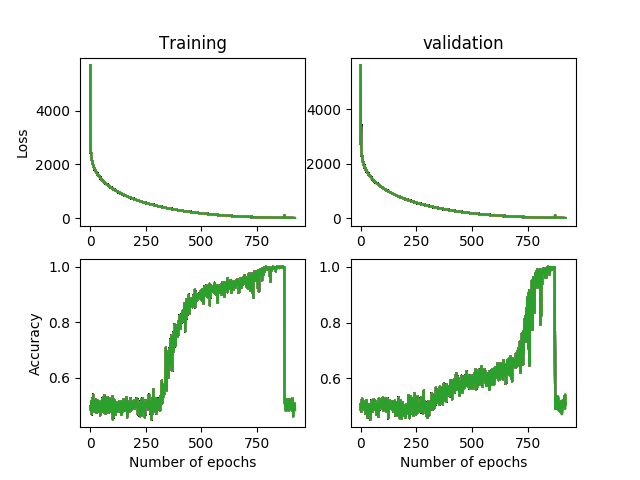
\includegraphics[scale=0.6]{test-batch2-1e-3-80-1e-2-5e-1}
\caption{Batch Size = 80, Learning Rate = 1e-3, Beta = 0.01, Dropout = 0.5}
\end{figure}
\item This run had an optimal validation accuracy of 99.7635 and an optimal test accuracy of 99.7297.  I also tested this multiple times, running the SAME set of hyperparameters, to see what is going on with that weird spike.  Does it keep showing up?  What is going on?  Here are more examples, all run at the same hyperparameters as above:
\begin{figure}[H]
\centering
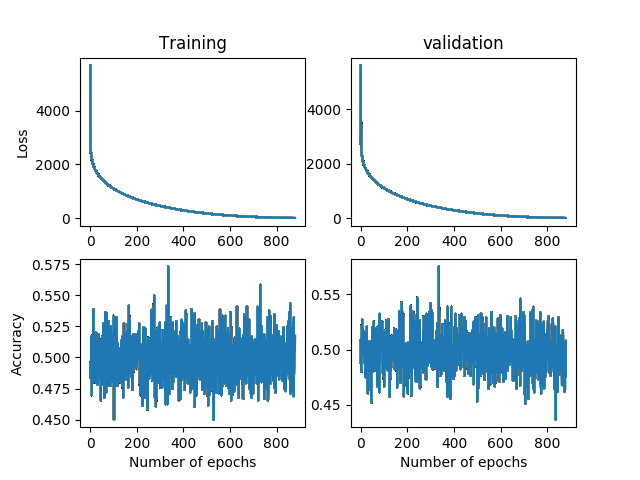
\includegraphics[scale=0.6]{learning-rate-rep1-1e-3-80-1e-2-5e-1}
\caption{Batch Size = 80, Learning Rate = 1e-3, Beta = 0.01, Dropout = 0.5}
\end{figure}
\item This run had an optimal validation accuracy of 47.0608, optimal test accuracy of 47.6689, and final validation accuracy of 49.223, test accuracy of 50.0338 

\begin{figure}[H]
\centering
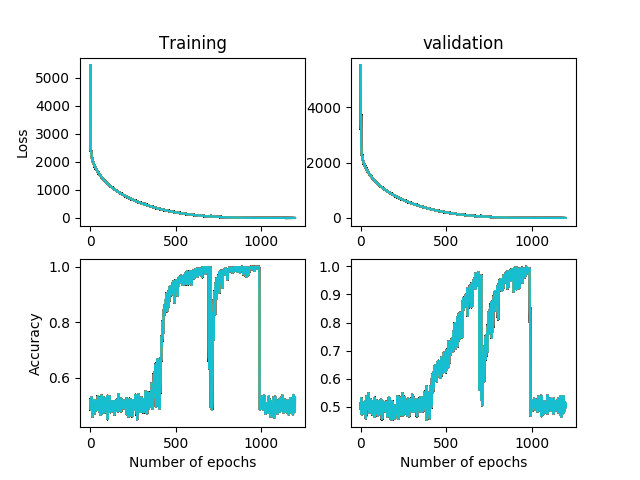
\includegraphics[scale=0.6]{learning-rate-rep2-1e-3-80-1e-2-5e-1}
\caption{Batch Size = 80, Learning Rate = 1e-3, Beta = 0.01, Dropout = 0.5}
\end{figure}
\item This run had an optimal validation accuracy of 99.4595, optimal test accuracy of 99.3243, and final validation accuracy of 50.777, test accuracy of 49.9662. 

\begin{figure}[H]
\centering
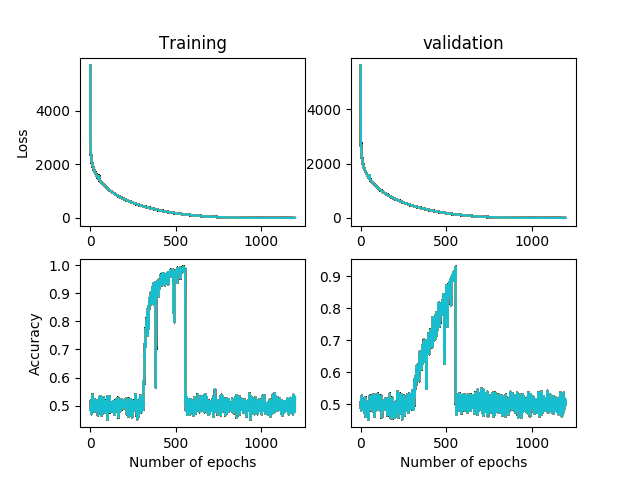
\includegraphics[scale=0.6]{learning-rate-rep3-1e-3-80-1e-2-5e-1}
\caption{Batch Size = 80, Learning Rate = 1e-3, Beta = 0.01, Dropout = 0.5}
\end{figure}
\item This run had an optimal validation accuracy of 992.5, optimal test accuracy of 91.7568, and final validation accuracy of 49.223, test accuracy of 50.0338. 

\begin{figure}[H]
\centering
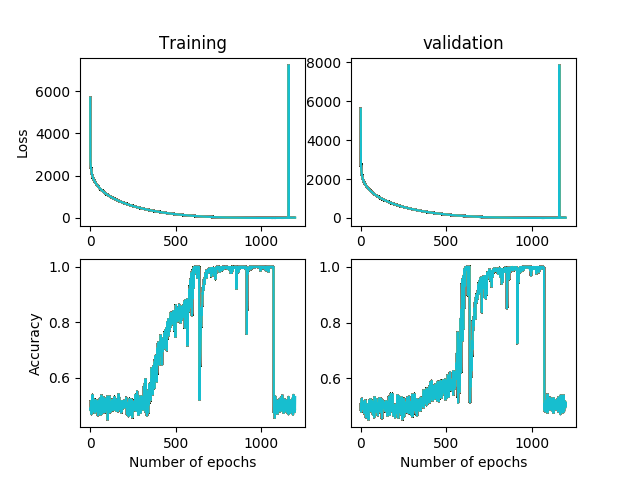
\includegraphics[scale=0.6]{learning-rate-rep4-1e-3-80-1e-2-5e-1}
\caption{Batch Size = 80, Learning Rate = 1e-3, Beta = 0.01, Dropout = 0.5}
\end{figure}
\item This run had an optimal validation accuracy of 99.8987, optimal test accuracy of 99.8649, and final validation accuracy of 50.777, test accuracy of 49.9662. 

\begin{figure}[H]
\centering
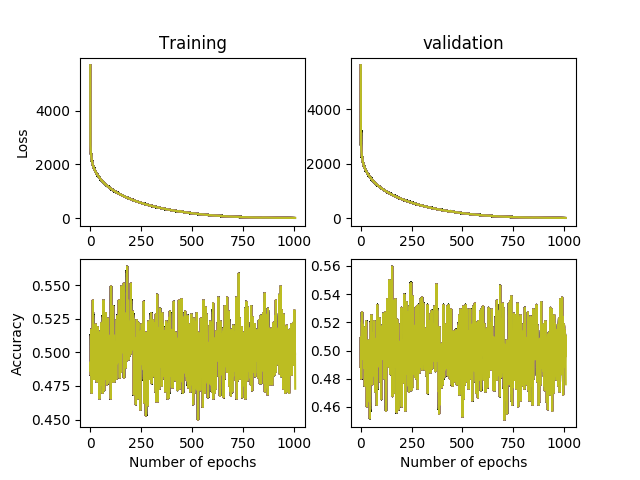
\includegraphics[scale=0.6]{learning-rate-rep5-1e-3-80-1e-2-5e-1}
\caption{Batch Size = 80, Learning Rate = 1e-3, Beta = 0.01, Dropout = 0.5}
\end{figure}
\item This run had an optimal validation accuracy of 55.4054, optimal test accuracy of 54.223, and final validation accuracy of 49,223, test accuracy of 50.0338.

\item The following are images of runs on the dataset that consists of glasses and liquids that are each 12 time steps away from the assumed glass transition temperature of 0.21.  

\begin{figure}[H]
\centering
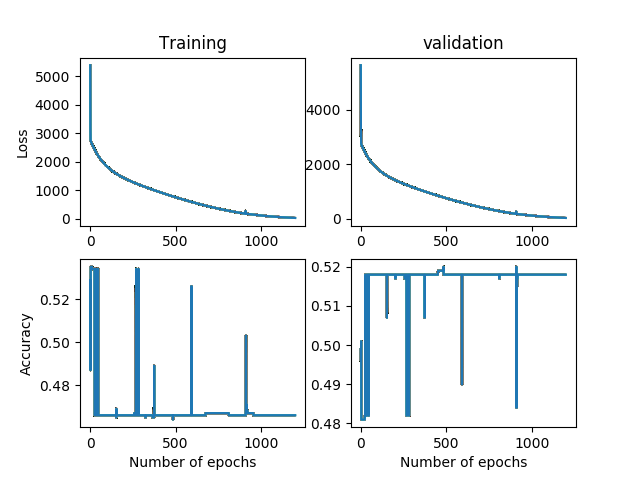
\includegraphics[scale=0.6]{data12-1e-4-100-1e-2-5e-1}
\caption{Batch Size = 100, Learning Rate = 1e-4, Beta = 0.01, Dropout = 0.5}
\end{figure}

\begin{figure}[H]
\centering
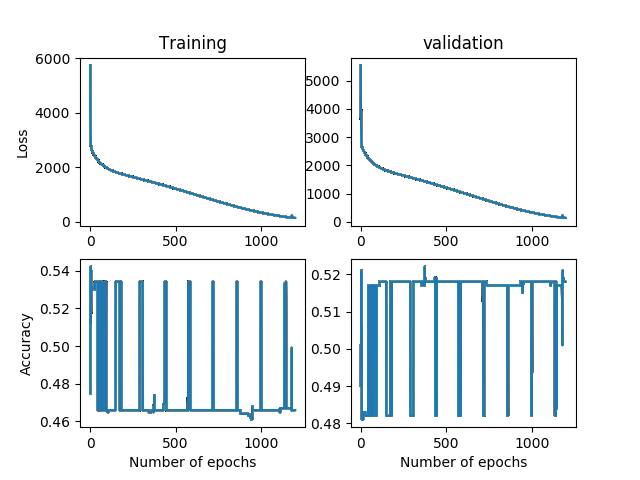
\includegraphics[scale=0.6]{data12-1e-4-10-1e-2-5e-1}
\caption{Batch Size = 10, Learning Rate = 1e-4, Beta = 0.01, Dropout = 0.5}
\end{figure}

\begin{figure}[H]
\centering
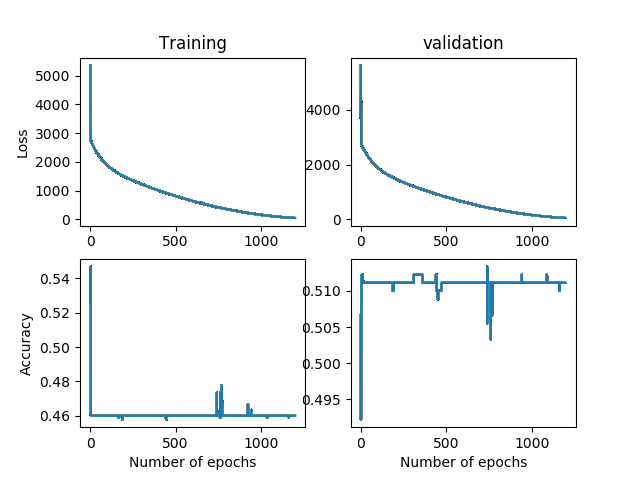
\includegraphics[scale=0.6]{data12-1e-4-150-1e-2-5e-1}
\caption{Batch Size = 150, Learning Rate = 1e-4, Beta = 0.01, Dropout = 0.5}
\end{figure}

\begin{figure}[H]
\centering
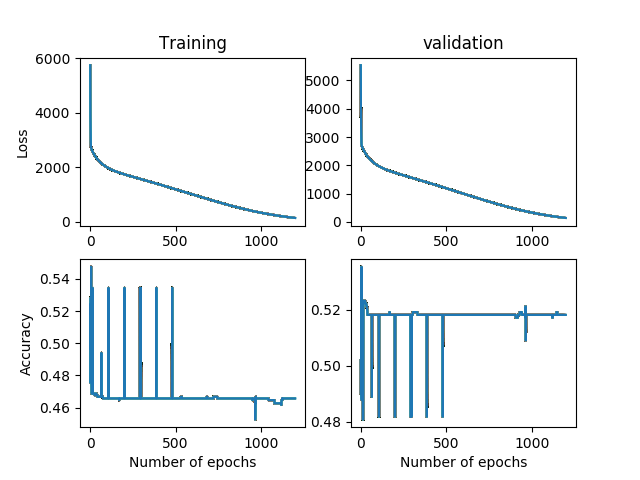
\includegraphics[scale=0.6]{data12-1e-4-15-1e-2-5e-1}
\caption{Batch Size = 15, Learning Rate = 1e-4, Beta = 0.01, Dropout = 0.5}
\end{figure}

\begin{figure}[H]
\centering
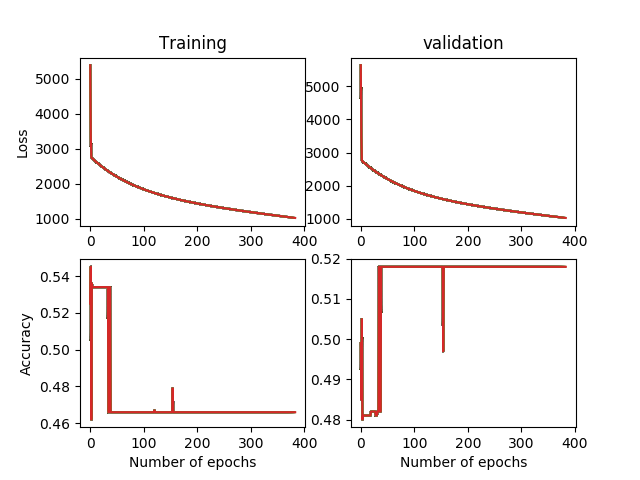
\includegraphics[scale=0.6]{data12-1e-4-200-1e-2-5e-1}
\caption{Batch Size = 200, Learning Rate = 1e-4, Beta = 0.01, Dropout = 0.5}
\end{figure}

\begin{figure}[H]
\centering
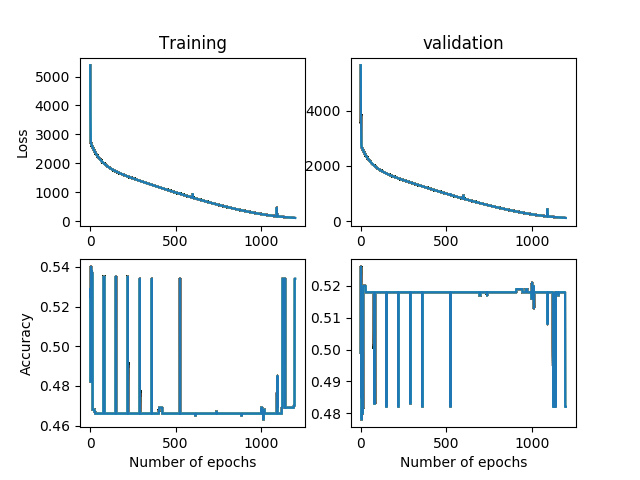
\includegraphics[scale=0.6]{data12-1e-4-20-1e-2-5e-1}
\caption{Batch Size = 20, Learning Rate = 1e-4, Beta = 0.01, Dropout = 0.5}
\end{figure}

\begin{figure}[H]
\centering
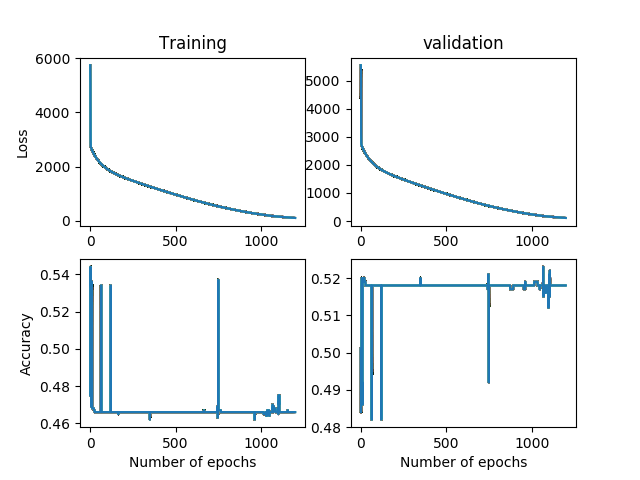
\includegraphics[scale=0.6]{data12-1e-4-25-1e-2-5e-1}
\caption{Batch Size = 25, Learning Rate = 1e-4, Beta = 0.01, Dropout = 0.5}
\end{figure}

\begin{figure}[H]
\centering
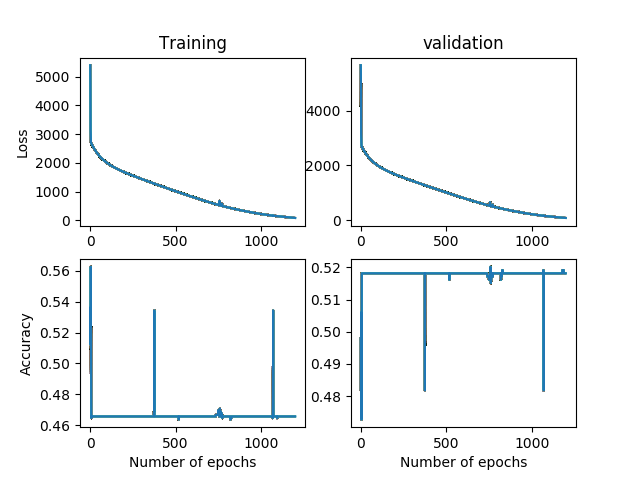
\includegraphics[scale=0.6]{data12-1e-4-30-1e-2-5e-1}
\caption{Batch Size = 30, Learning Rate = 1e-4, Beta = 0.01, Dropout = 0.5}
\end{figure}

\begin{figure}[H]
\centering
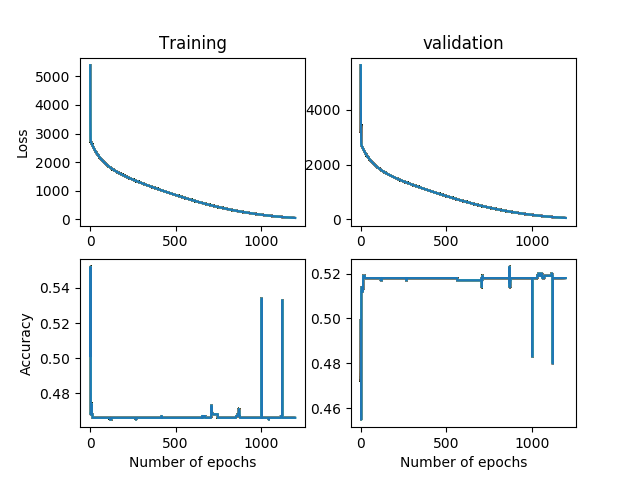
\includegraphics[scale=0.6]{data12-1e-4-50-1e-2-5e-1}
\caption{Batch Size = 50, Learning Rate = 1e-4, Beta = 0.01, Dropout = 0.5}
\end{figure}

\begin{figure}[H]
\centering
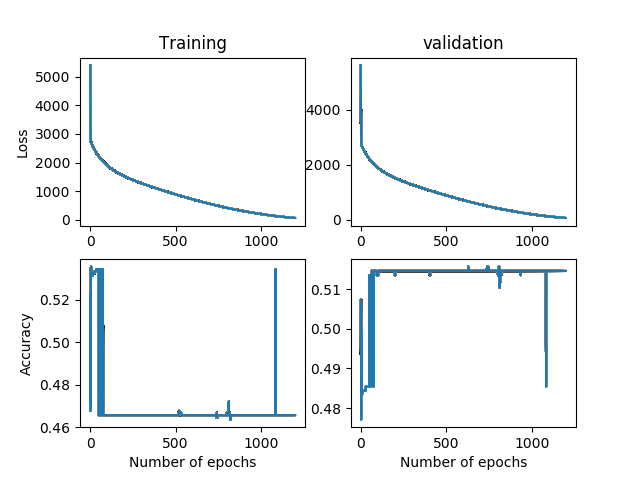
\includegraphics[scale=0.6]{data12-1e-4-80-1e-2-5e-1}
\caption{Batch Size = 80, Learning Rate = 1e-4, Beta = 0.01, Dropout = 0.5}
\end{figure}

\begin{figure}[H]
\centering
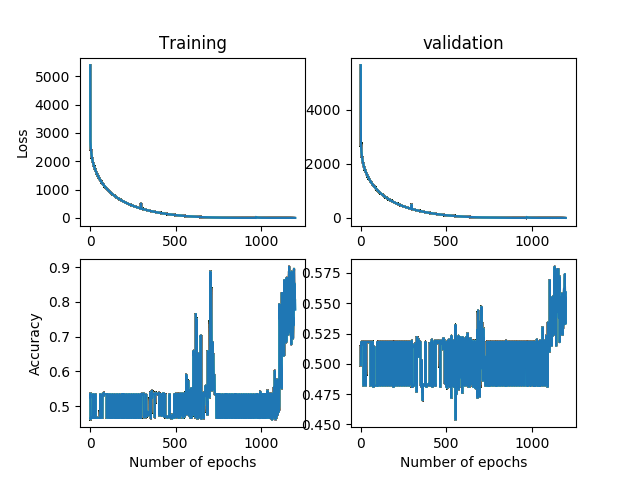
\includegraphics[scale=0.6]{data12-1e-3-100-1e-2-5e-1}
\caption{Batch Size = 100, Learning Rate = 1e-3, Beta = 0.01, Dropout = 0.5}
\end{figure}

\begin{figure}[H]
\centering
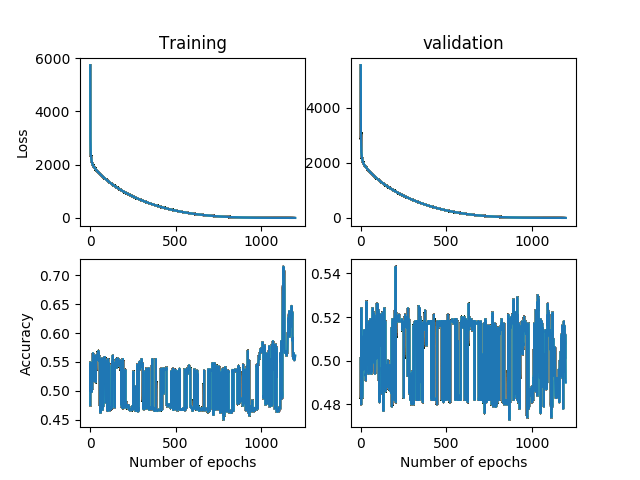
\includegraphics[scale=0.6]{data12-1e-3-10-1e-2-5e-1}
\caption{Batch Size = 10, Learning Rate = 1e-3, Beta = 0.01, Dropout = 0.5}
\end{figure}

\begin{figure}[H]
\centering
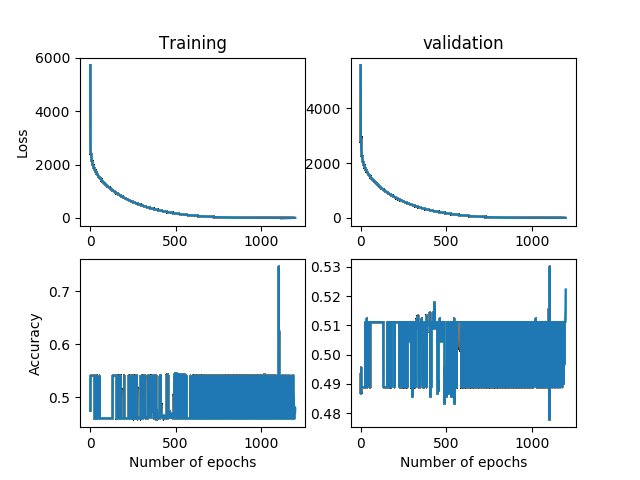
\includegraphics[scale=0.6]{data12-1e-3-150-1e-2-5e-1}
\caption{Batch Size = 150, Learning Rate = 1e-3, Beta = 0.01, Dropout = 0.5}
\end{figure}

\begin{figure}[H]
\centering
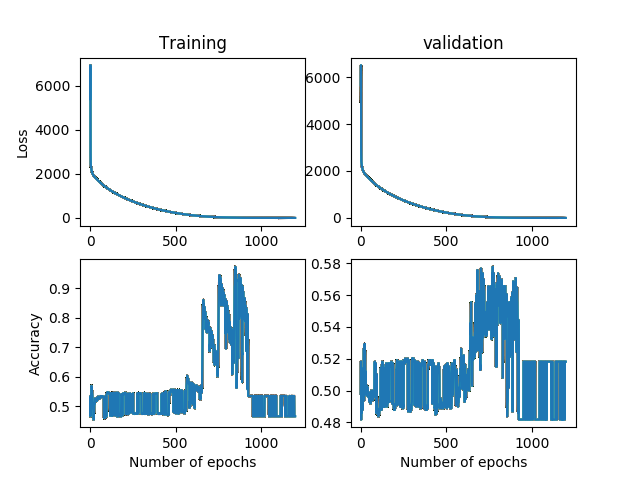
\includegraphics[scale=0.6]{data12-1e-3-15-1e-2-5e-1}
\caption{Batch Size = 15, Learning Rate = 1e-3, Beta = 0.01, Dropout = 0.5}
\end{figure}

\begin{figure}[H]
\centering
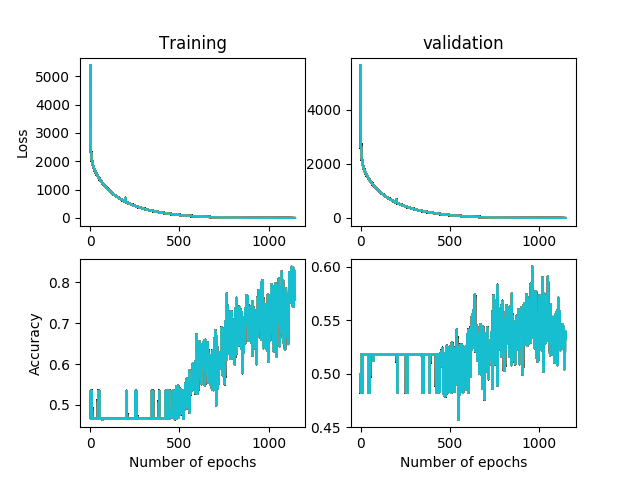
\includegraphics[scale=0.6]{data12-1e-3-200-1e-2-1e-1}
\caption{Batch Size = 200, Learning Rate = 1e-3, Beta = 0.01, Dropout = 0.1}
\end{figure}

\begin{figure}[H]
\centering
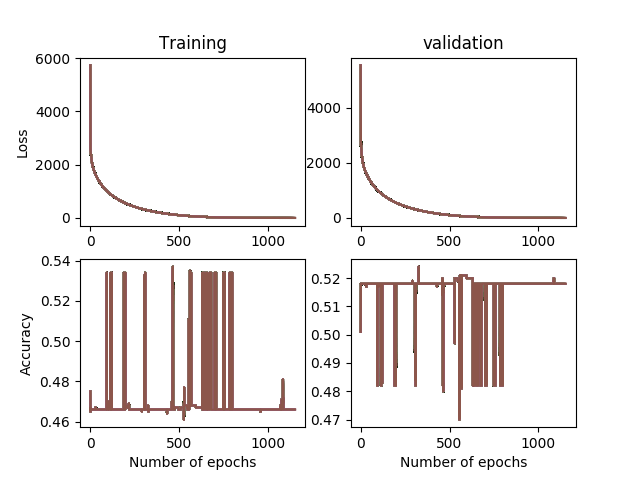
\includegraphics[scale=0.6]{data12-1e-3-200-1e-2-2e-1}
\caption{Batch Size = 200, Learning Rate = 1e-3, Beta = 0.01, Dropout = 0.2}
\end{figure}

\begin{figure}[H]
\centering
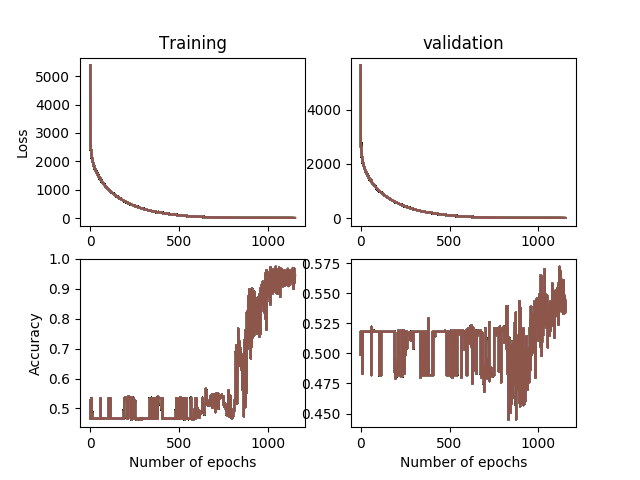
\includegraphics[scale=0.6]{data12-1e-3-200-1e-2-3e-1}
\caption{Batch Size = 200, Learning Rate = 1e-3, Beta = 0.01, Dropout = 0.3}
\end{figure}

\begin{figure}[H]
\centering
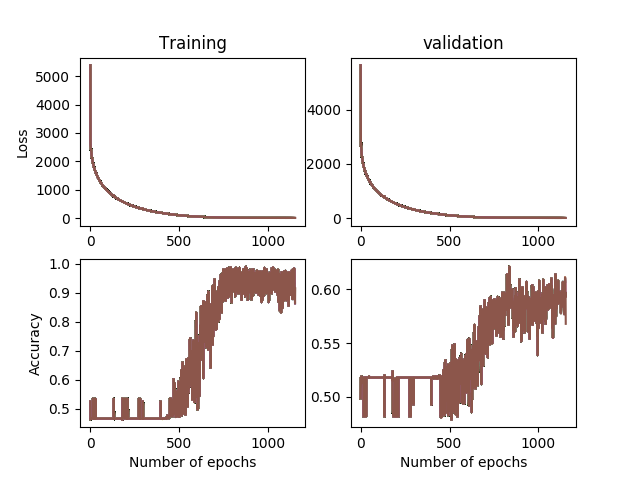
\includegraphics[scale=0.6]{data12-1e-3-200-1e-2-4e-1}
\caption{Batch Size = 200, Learning Rate = 1e-3, Beta = 0.01, Dropout = 0.4}
\end{figure}

\begin{figure}[H]
\centering
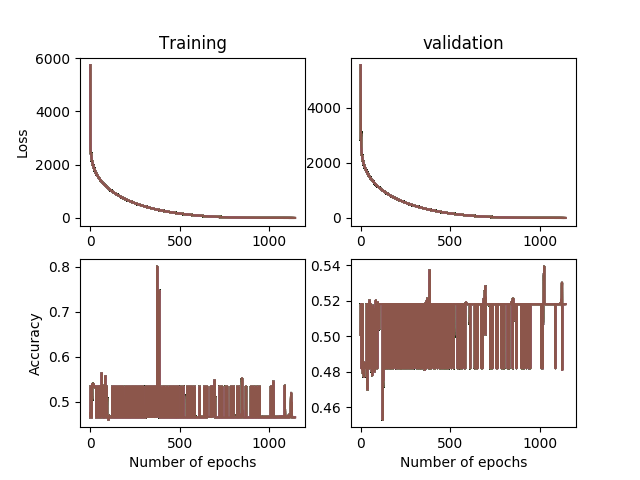
\includegraphics[scale=0.6]{data12-1e-3-200-1e-2-5e-1}
\caption{Batch Size = 200, Learning Rate = 1e-3, Beta = 0.01, Dropout = 0.5}
\end{figure}

\begin{figure}[H]
\centering
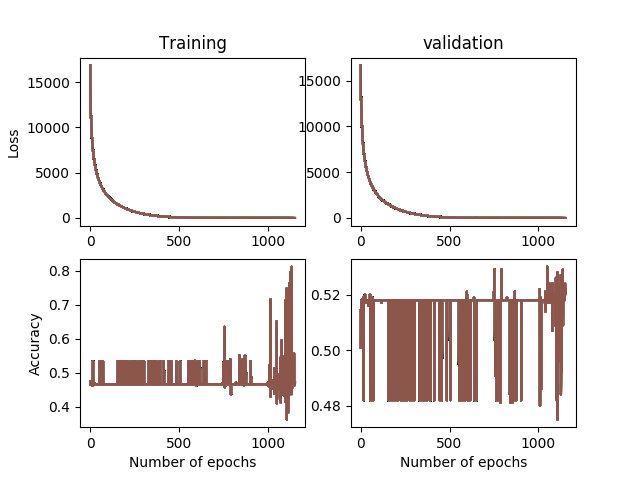
\includegraphics[scale=0.6]{data12-1e-3-200-5e-2-3e-1}
\caption{Batch Size = 200, Learning Rate = 1e-3, Beta = 0.01, Dropout = 0.3}
\end{figure}

\begin{figure}[H]
\centering
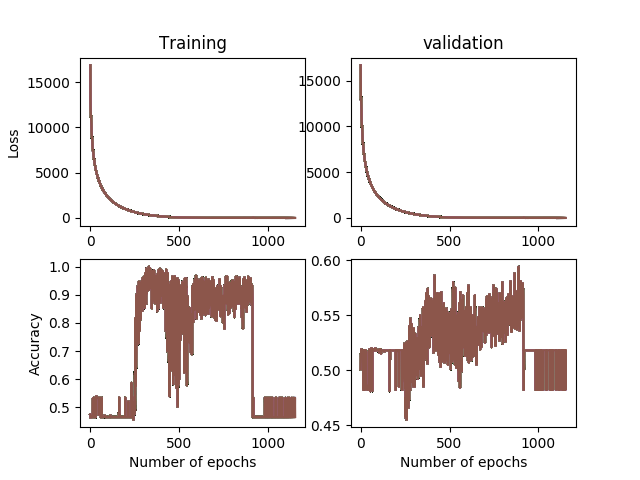
\includegraphics[scale=0.6]{data12-1e-3-200-5e-2-4e-1}
\caption{Batch Size = 200, Learning Rate = 1e-3, Beta = 0.01, Dropout = 0.4}
\end{figure}

\begin{figure}[H]
\centering
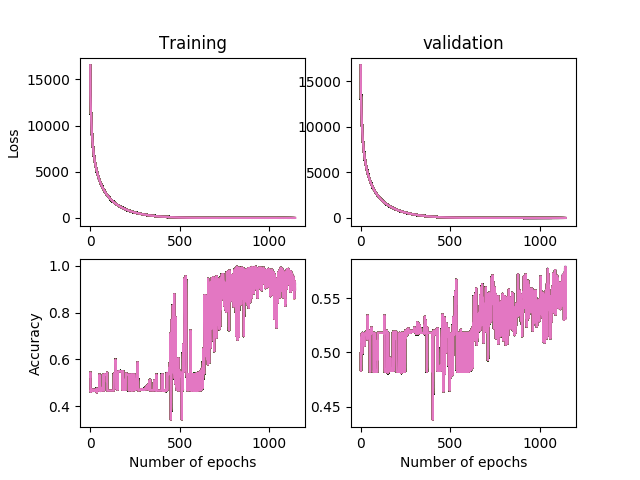
\includegraphics[scale=0.6]{data12-1e-3-200-5e-2-5e-1}
\caption{Batch Size = 200, Learning Rate = 1e-3, Beta = 0.01, Dropout = 0.4}
\end{figure}

\begin{figure}[H]
\centering
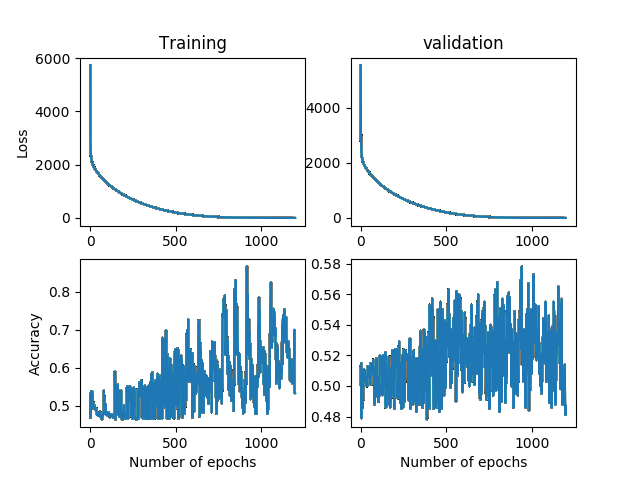
\includegraphics[scale=0.6]{data12-1e-3-20-1e-2-5e-1}
\caption{Batch Size = 20, Learning Rate = 1e-3, Beta = 0.01, Dropout = 0.5}
\end{figure}

\begin{figure}[H]
\centering
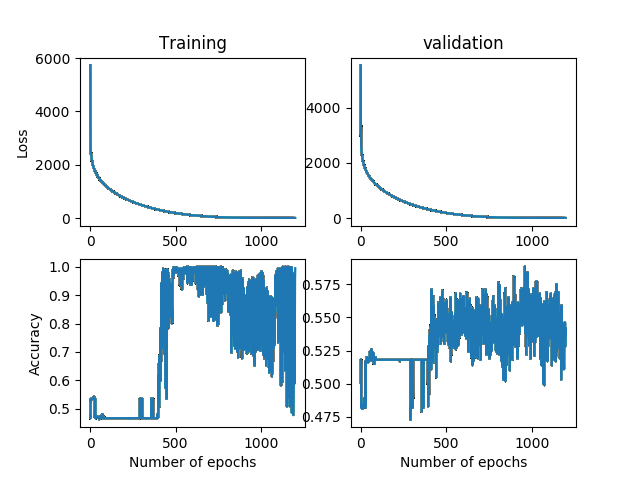
\includegraphics[scale=0.6]{data12-1e-3-250-1e-2-5e-1}
\caption{Batch Size = 250, Learning Rate = 1e-3, Beta = 0.01, Dropout = 0.5}
\end{figure}

\begin{figure}[H]
\centering
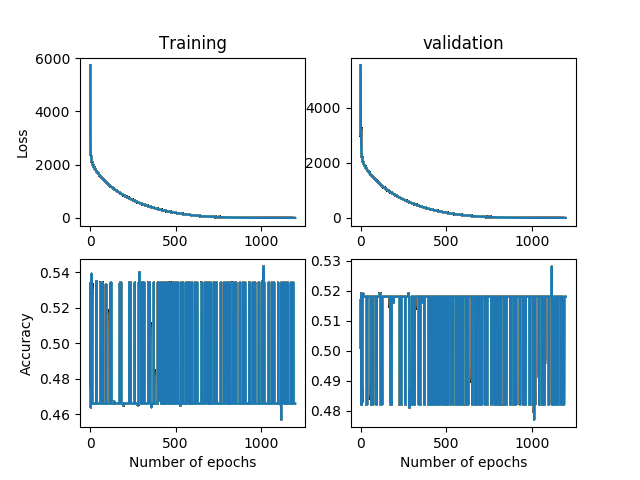
\includegraphics[scale=0.6]{data12-1e-3-25-1e-2-5e-1}
\caption{Batch Size = 25, Learning Rate = 1e-3, Beta = 0.01, Dropout = 0.5}
\end{figure}

\begin{figure}[H]
\centering
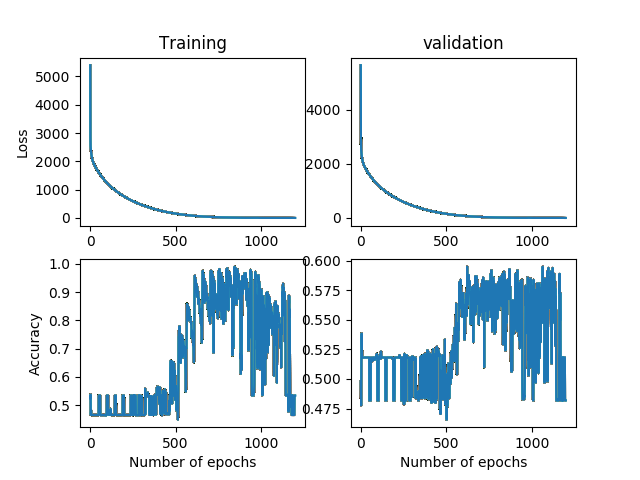
\includegraphics[scale=0.6]{data12-1e-3-30-1e-2-5e-1}
\caption{Batch Size = 30, Learning Rate = 1e-3, Beta = 0.01, Dropout = 0.5}
\end{figure}

\begin{figure}[H]
\centering
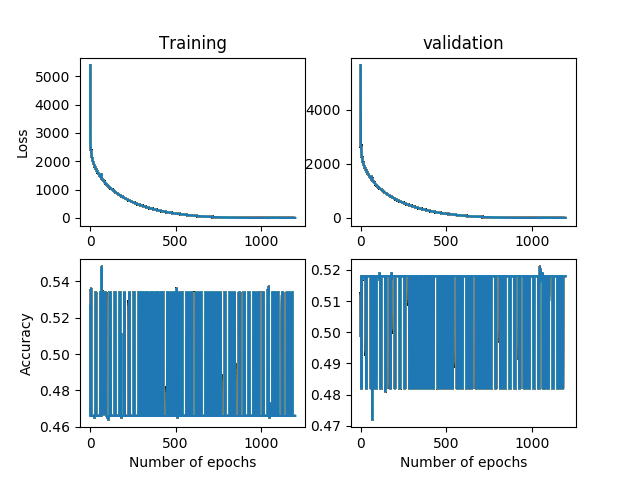
\includegraphics[scale=0.6]{data12-1e-3-50-1e-2-5e-1}
\caption{Batch Size = 50, Learning Rate = 1e-3, Beta = 0.01, Dropout = 0.5}
\end{figure}

\item Visualizations.  
\begin{figure}[H]
\centering
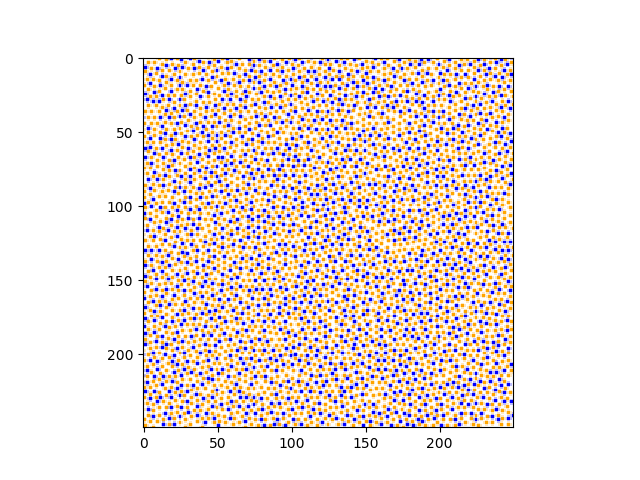
\includegraphics[scale=0.6]{glass_original}
\caption{Glass original}
\end{figure}

\begin{figure}[H]
\centering
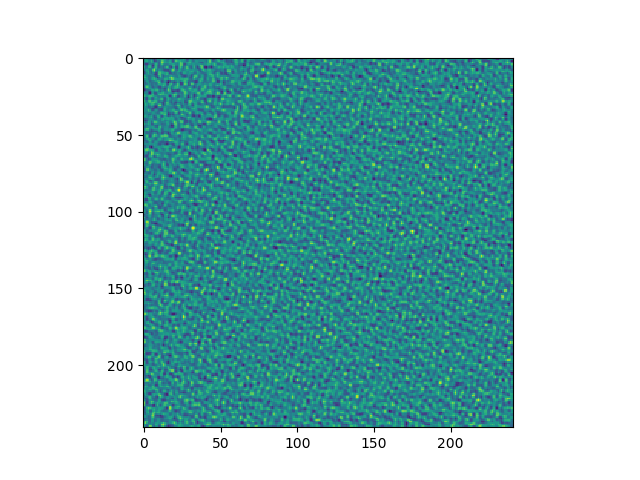
\includegraphics[scale=0.6]{glass_channel_1}
\caption{Glass channel 1}
\end{figure}

\begin{figure}[H]
\centering
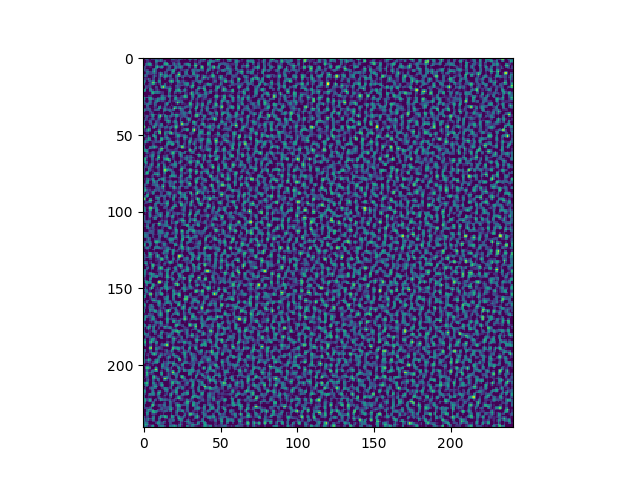
\includegraphics[scale=0.6]{glass_channel_2}
\caption{Glass channel 2}
\end{figure}

\begin{figure}[H]
\centering
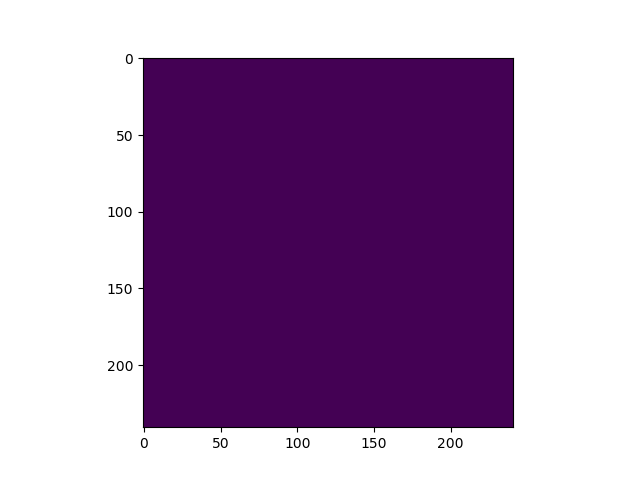
\includegraphics[scale=0.6]{glass_channel_3}
\caption{Glass channel 3}
\end{figure}

\begin{figure}[H]
\centering
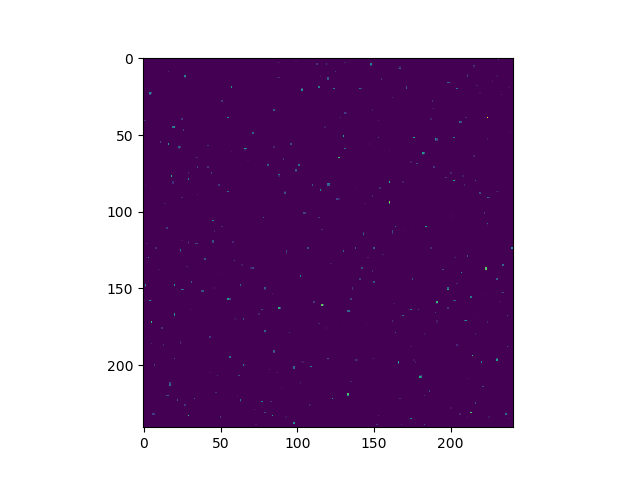
\includegraphics[scale=0.6]{glass_channel_4}
\caption{Glass channel 4}
\end{figure}

\begin{figure}[H]
\centering
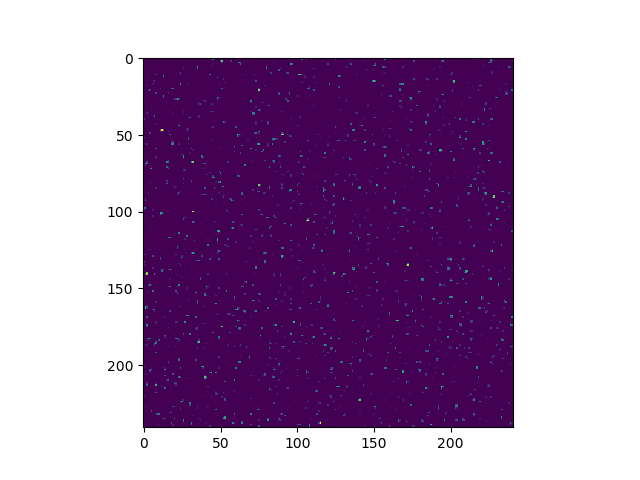
\includegraphics[scale=0.6]{glass_channel_5}
\caption{Glass channel 5}
\end{figure}

\begin{figure}[H]
\centering
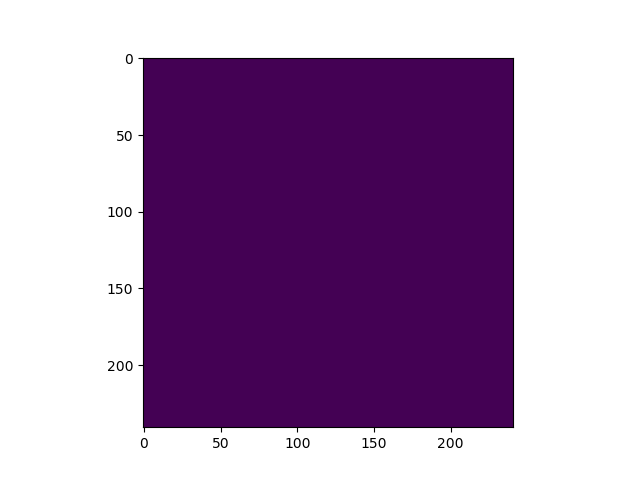
\includegraphics[scale=0.6]{glass_channel_6}
\caption{Glass channel 6}
\end{figure}

\begin{figure}[H]
\centering
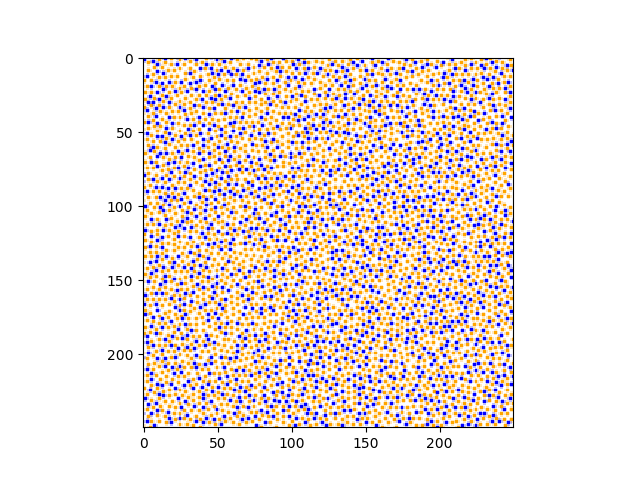
\includegraphics[scale=0.6]{liquid_original}
\caption{Liquid original}
\end{figure}

\begin{figure}[H]
\centering
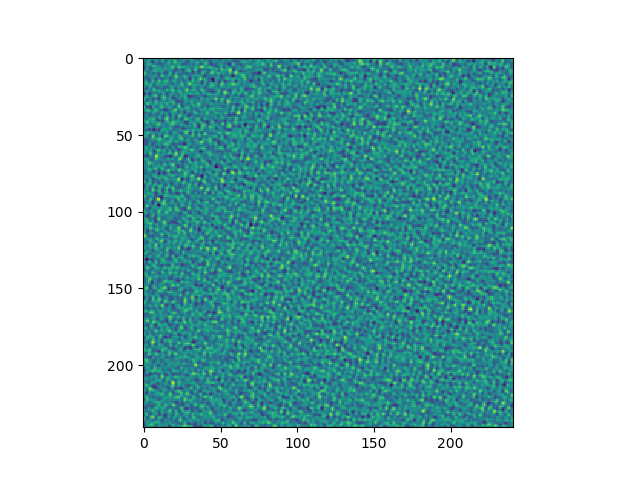
\includegraphics[scale=0.6]{liquid_channel_1}
\caption{Liquid channel 1}
\end{figure}

\begin{figure}[H]
\centering
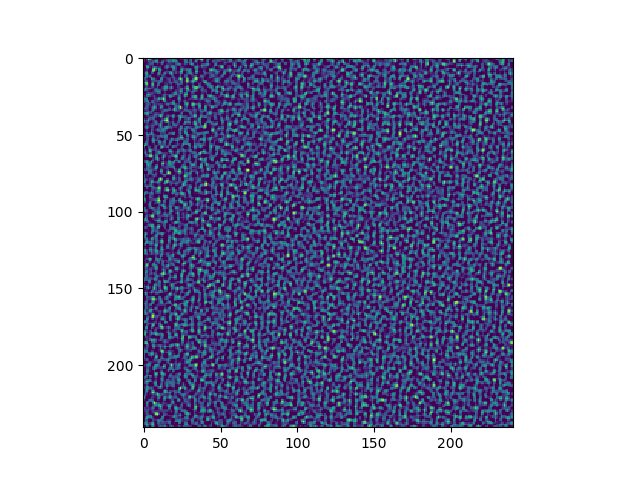
\includegraphics[scale=0.6]{liquid_channel_2}
\caption{Liquid channel 2}
\end{figure}

\begin{figure}[H]
\centering
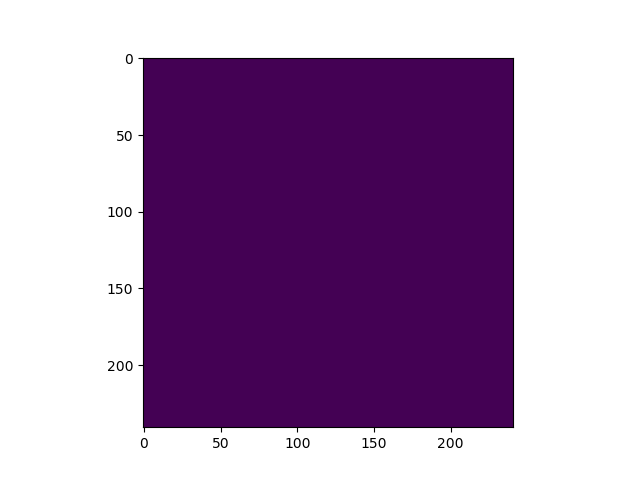
\includegraphics[scale=0.6]{liquid_channel_3}
\caption{Liquid channel 3}
\end{figure}

\begin{figure}[H]
\centering
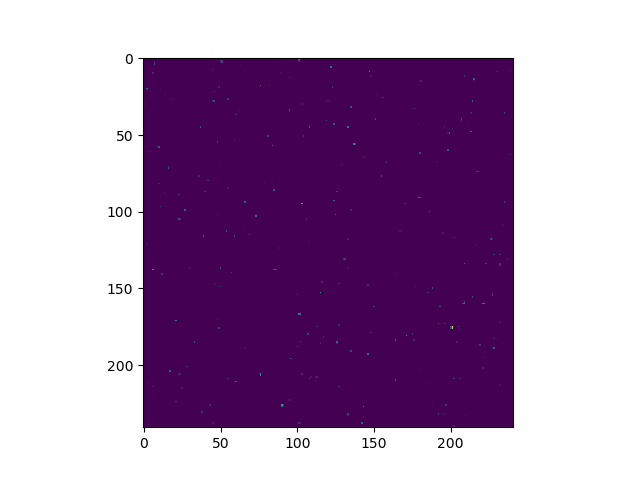
\includegraphics[scale=0.6]{liquid_channel_4}
\caption{Liquid channel 4}
\end{figure}

\begin{figure}[H]
\centering
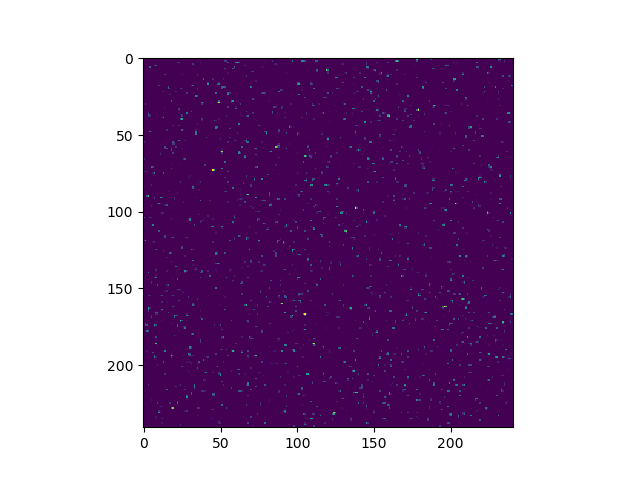
\includegraphics[scale=0.6]{liquid_channel_5}
\caption{Liquid channel 5}
\end{figure}

\begin{figure}[H]
\centering
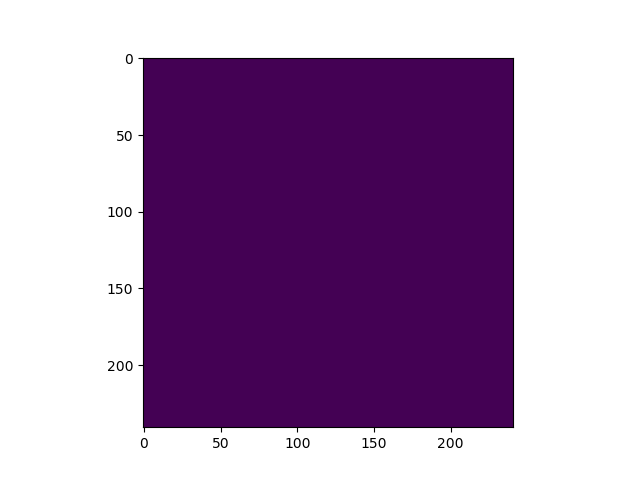
\includegraphics[scale=0.6]{liquid_channel_6}
\caption{Liquid channel 6}
\end{figure}

\end{enumerate}

\section{12/13/2017}
\begin{enumerate}
\item Updated python scripts and merged with GitHub - the recent additions include streamlining the learning rate schedule and data augmentation options.  The following is for a standard run on the original endpoint data:

\begin{figure}[H]
\centering
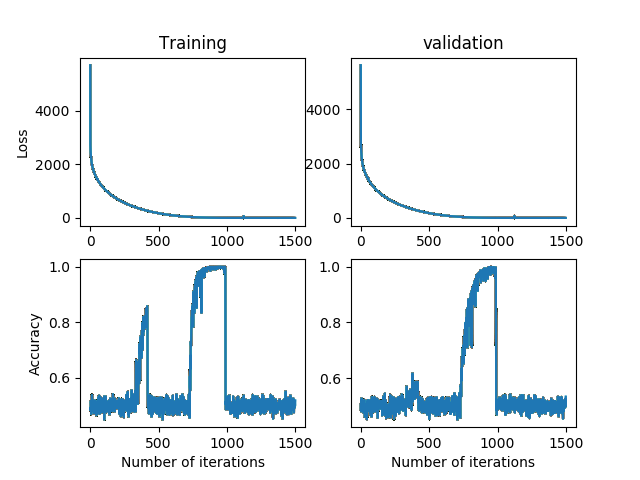
\includegraphics[scale=0.6]{test-1e-3-1e-3-550-80-1e-2-5e-1}
\caption{Initial Learning Rate = 1e-3, Final Learning Rate = 1e-3, Schedule Length = 550 iterations, Batch Size = 80, L2 beta = 0.01, Dropout = 0.5}
\end{figure}

\item I then, twice, set the final learning rate to be smaller, at 1e-4:

\begin{figure}[H]
\centering
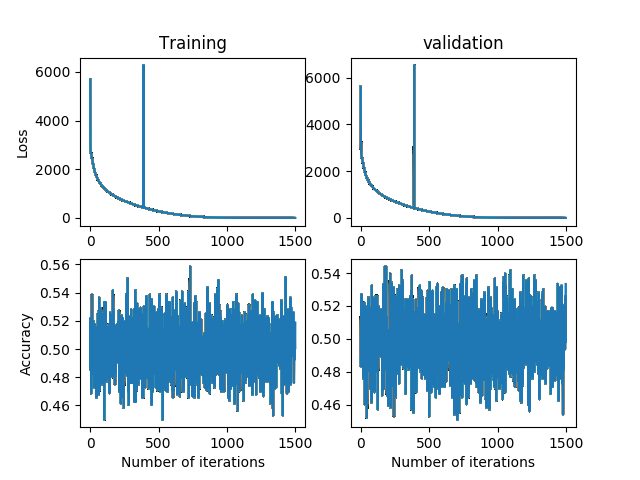
\includegraphics[scale=0.6]{test-1e-4-1e-3-550-80-1e-2-5e-1}
\caption{Initial Learning Rate = 1e-3, Final Learning Rate = 1e-3, Schedule Length = 550 iterations, Batch Size = 80, L2 beta = 0.01, Dropout = 0.5}
\end{figure}

\begin{figure}[H]
\centering
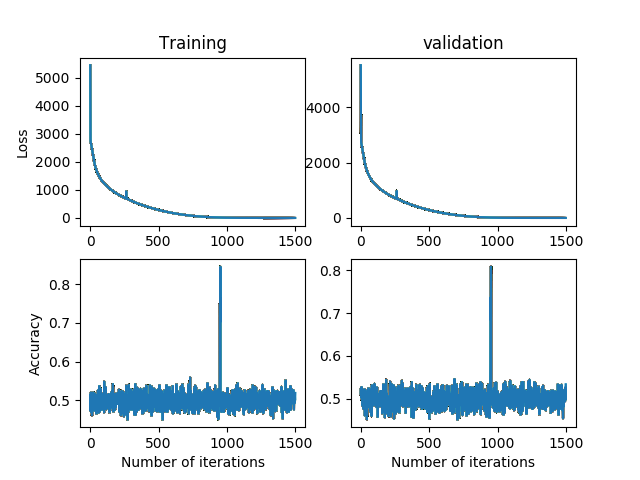
\includegraphics[scale=0.6]{test2-1e-4-1e-3-550-80-1e-2-5e-1}
\caption{Initial Learning Rate = 1e-3, Final Learning Rate = 1e-3, Schedule Length = 550 iterations, Batch Size = 80, L2 beta = 0.01, Dropout = 0.5}
\end{figure}

\item What is going on here?  It seems as though setting the learning rate a magnitude lower really screws things up...
\item Note: one iteration goes through 10 batches, so if the batch size is 80, then one iteration goes through 800 examples.  The training set is 70 percent of the total 20,000 images, so the training set is 14,000 images.  Thus, one epoch is 17.5 iterations, or approximately 18 iterations.  That means that 1500 iterations is about 83 epochs.  Question: how many epochs is typically needed for a binary classification problem?  And how long does this typically take?
\item I also tested the usual hyperparameters on the original endpoint data and turned on the data augmentation, to see if there would be any issues.  I got the following training runs:

\begin{figure}[H]
\centering
\includegraphics[scale=0.6]{data_aug}
\caption{Initial Learning Rate = NA, Final Learning Rate = 1e-3, Schedule Length = NA, Batch Size = 80, L2 beta = 0.01, Dropout = 0.5}
\end{figure}

\begin{figure}[H]
\centering
\includegraphics[scale=0.6]{data_aug2}
\caption{Initial Learning Rate = NA, Final Learning Rate = 1e-3, Schedule Length = NA, Batch Size = 80, L2 beta = 0.01, Dropout = 0.5}
\end{figure}

\begin{figure}[H]
\centering
\includegraphics[scale=0.6]{data_aug3}
\caption{Initial Learning Rate = NA, Final Learning Rate = 1e-3, Schedule Length = NA, Batch Size = 80, L2 beta = 0.01, Dropout = 0.5}
\end{figure}

\begin{figure}[H]
\centering
\includegraphics[scale=0.6]{data_aug4}
\caption{Initial Learning Rate = NA, Final Learning Rate = 1e-3, Schedule Length = NA, Batch Size = 80, L2 beta = 0.01, Dropout = 0.5}
\end{figure}

\begin{figure}[H]
\centering
\includegraphics[scale=0.6]{data_aug5}
\caption{Initial Learning Rate = NA, Final Learning Rate = 1e-3, Schedule Length = NA, Batch Size = 80, L2 beta = 0.01, Dropout = 0.5}
\end{figure}

\item I should double check that the dataset augmentation is actually working.  
\end{enumerate}
\section{12/22/2017}
\begin{enumerate}
\item I am now going to run a series of training runs that will explore the relationship between the learning rate schedule and accuracy.  First, let's try the threshold idea.  Then, we will try the standard exponential decay idea.  Let's try the following.  When the accuracy gets to 90 percent, let's decrease the learning rate by an order of magnitude.  Let's just run that simple test, say, 8 times, and see what happens!

\item Initial learning rate = , Final learning rate = ,   
\end{enumerate}
\section{12/24/2017}
\begin{enumerate}
\item We ran a series of training runs that used a learning rate threshold.  The learning rate starts at the initial learning rate.  The learning rate changes to the final learning rate whenever the validation accuracy is above 90 percent.  This allows the learning rate to go back to the initial learning rate if the accuracy drops below 90 percent.  Here are plots showing six tests.  These plots demonstrate that the sharp drops in accuracy were, indeed, the result of a learning rate that was too large towards the end of training, since there are no sharp drops in accuracy here:

\begin{figure}[H]
\centering
\includegraphics[scale=0.6]{threshold-test-1e-3-1e-4-1}
\caption{Initial Learning Rate = 1e-3, Final Learning Rate = 1e-4, Schedule Length = NA, Batch Size = 80, L2 beta = 0.01, Dropout = 0.5}
\end{figure}

\begin{figure}[H]
\centering
\includegraphics[scale=0.6]{threshold-test-1e-3-1e-4-2}
\caption{Initial Learning Rate = 1e-3, Final Learning Rate = 1e-4, Schedule Length = NA, Batch Size = 80, L2 beta = 0.01, Dropout = 0.5}
\end{figure}

\begin{figure}[H]
\centering
\includegraphics[scale=0.6]{threshold-test-1e-3-1e-4-3}
\caption{Initial Learning Rate = 1e-3, Final Learning Rate = 1e-4, Schedule Length = NA, Batch Size = 80, L2 beta = 0.01, Dropout = 0.5}
\end{figure}

\begin{figure}[H]
\centering
\includegraphics[scale=0.6]{threshold-test-1e-3-1e-5-1}
\caption{Initial Learning Rate = 1e-3, Final Learning Rate = 1e-4, Schedule Length = NA, Batch Size = 80, L2 beta = 0.01, Dropout = 0.5}
\end{figure}

\begin{figure}[H]
\centering
\includegraphics[scale=0.6]{threshold-test-1e-3-1e-5-2}
\caption{Initial Learning Rate = 1e-3, Final Learning Rate = 1e-4, Schedule Length = NA, Batch Size = 80, L2 beta = 0.01, Dropout = 0.5}
\end{figure}

\begin{figure}[H]
\centering
\includegraphics[scale=0.6]{threshold-test-1e-3-1e-5-3}
\caption{Initial Learning Rate = 1e-3, Final Learning Rate = 1e-4, Schedule Length = NA, Batch Size = 80, L2 beta = 0.01, Dropout = 0.5}
\end{figure}

\end{enumerate}

\subsection{12/29/2017}
\begin{enumerate}
\item Ran another series of runs that used a similar learning rate threshold just to check that my GitHub had been updated appropriately.  This time used only 1e-3 to 1e-4.  In one example, the accuracy crashed.  Perhaps evidences that smaller learning rates are needed closer to the minimum.  For the sake of completeness, these extra runs are reported below:  

\begin{figure}[H]
\centering
\includegraphics[scale=0.6]{Commit-test-1}
\caption{Initial Learning Rate = 1e-3, Final Learning Rate = 1e-4, Schedule Length = NA, Batch Size = 80, L2 beta = 0.01, Dropout = 0.5}
\end{figure}

\begin{figure}[H]
\centering
\includegraphics[scale=0.6]{Commit-test-2}
\caption{Initial Learning Rate = 1e-3, Final Learning Rate = 1e-4, Schedule Length = NA, Batch Size = 80, L2 beta = 0.01, Dropout = 0.5}
\end{figure}

\begin{figure}[H]
\centering
\includegraphics[scale=0.6]{Commit-test-3}
\caption{Initial Learning Rate = 1e-3, Final Learning Rate = 1e-4, Schedule Length = NA, Batch Size = 80, L2 beta = 0.01, Dropout = 0.5}
\end{figure}

\begin{figure}[H]
\centering
\includegraphics[scale=0.6]{Commit-test-4}
\caption{Initial Learning Rate = 1e-3, Final Learning Rate = 1e-4, Schedule Length = NA, Batch Size = 80, L2 beta = 0.01, Dropout = 0.5}
\end{figure}

\begin{figure}[H]
\centering
\includegraphics[scale=0.6]{Commit-test-5}
\caption{Initial Learning Rate = 1e-3, Final Learning Rate = 1e-4, Schedule Length = NA, Batch Size = 80, L2 beta = 0.01, Dropout = 0.5}
\end{figure}

\begin{figure}[H]
\centering
\includegraphics[scale=0.6]{Commit-test-6}
\caption{Initial Learning Rate = 1e-3, Final Learning Rate = 1e-4, Schedule Length = NA, Batch Size = 80, L2 beta = 0.01, Dropout = 0.5}
\end{figure}

\begin{figure}[H]
\centering
\includegraphics[scale=0.6]{Commit-test-7}
\caption{Initial Learning Rate = 1e-3, Final Learning Rate = 1e-4, Schedule Length = NA, Batch Size = 80, L2 beta = 0.01, Dropout = 0.5}
\end{figure}


\end{enumerate}

\subsection{12/30/2017}
\begin{enumerate}
\item Tested the data augmentation scheme manually.  Printed out a series of images and their respective augmented versions that are given when generator.next is invoked, respectively with the data aug option set to false and with the data aug option set to true.  

\end{enumerate}

\subsection{1/1/2018}
\begin{enumerate}
\item Added main\_glassliquid\_restart.py, a file that can run training starting from a previous saved model.  Tested it.  Now, let's try to train again on the dataset that consists of glasses and liquids that are each 12 time steps away from the assumed glass transition temperature of 0.21.  Previously, the best parameters were batch size 200, learning rate 1e-3, beta 0.01, dropout 0.4.  Now, we are going to do a series of simulations using the same parameters, except, first, we are going to include dataset augmentation, and second, we are going to run the simluation at least twice as long.  Then, once we get a sense for how these train, we will add in a learning rate threshold step, or even multiple threshold steps if necessary!     

\end{enumerate}

\subsection{1/4/2018}
\begin{enumerate}
\item Realized that I had run on the original endpoint data.  So, copied over the folder called "data\_12steps" into the current machine-learning-glasses directory, removed the current metadata folder, and created a new metadata folder with this data.  Then, set up new training runs again.      

\end{enumerate}

\section{1/9/2018}
\begin{enumerate}
\item Collected data from the above-mentioned simulations.  The training curves are as follows:

\begin{figure}[H]
\centering
\includegraphics[scale=0.6]{data12_version1_step0}
\caption{Version 1: Initial Learning Rate = 1e-3, Final Learning Rate = 1e-4, Schedule Length = NA, Batch Size = 80, L2 beta = 0.01, Dropout = 0.4, data aug = true}
\end{figure}

\begin{figure}[H]
\centering
\includegraphics[scale=0.6]{data12_version2_step0}
\caption{Version 2: Initial Learning Rate = 1e-3, Final Learning Rate = 1e-4, Schedule Length = NA, Batch Size = 80, L2 beta = 0.01, Dropout = 0.4, data aug = true}
\end{figure}

\begin{figure}[H]
\centering
\includegraphics[scale=0.6]{data12_version3_step0}
\caption{Version 3: Initial Learning Rate = 1e-3, Final Learning Rate = 1e-4, Schedule Length = NA, Batch Size = 80, L2 beta = 0.01, Dropout = 0.4, data aug = true}
\end{figure}

\begin{figure}[H]
\centering
\includegraphics[scale=0.6]{data12_version4_step0}
\caption{Version 4: Initial Learning Rate = 1e-3, Final Learning Rate = 1e-4, Schedule Length = NA, Batch Size = 80, L2 beta = 0.01, Dropout = 0.4, data aug = true}
\end{figure}

\begin{figure}[H]
\centering
\includegraphics[scale=0.6]{data12_version5_step0}
\caption{Version 5: Initial Learning Rate = 1e-3, Final Learning Rate = 1e-4, Schedule Length = NA, Batch Size = 80, L2 beta = 0.01, Dropout = 0.4, data aug = true}
\end{figure}

\begin{figure}[H]
\centering
\includegraphics[scale=0.6]{data12_version6_step0}
\caption{Version 6: Initial Learning Rate = 1e-3, Final Learning Rate = 1e-4, Schedule Length = NA, Batch Size = 80, L2 beta = 0.01, Dropout = 0.4, data aug = true}
\end{figure}

\item The problem is that my allotted time (36 hours) was not enough, so the simulations terminated early.  My program, however, was only set to save the current model at the end of the iterations.  So, the current model was not saved, only the best model was saved.  So, I went back into the main code and changed it so that the current model is updated and saved at every iteration, in addition to the best model being updated when necessary.  I also included restart capability into the main code (using parsing options), so that there is not a separate restart file.  

\item I am now running 7 new simulations.  The first is just a re-do of version1 step 0.  The others take version5 step 0 and start from the saved best model as a starting point, using the new restart capabilities of the main code.  The first two simulations from this starting point (version5 step2 and version5 step2 trial2) use the original parameters.  The next two (version5 step2 trial3 and version5 step2 trial4 use eta\_initial=1e-4 and eta\_final=1e-5), and the final two (version5 step2 trial5 and version5 step2 trial6) use eta\_intial=1e-5 and eta\_final=1e-6.  We will see how these 7 new runs turn out.  
\end{enumerate}

\subsection{1/14/2018}
\begin{enumerate}
\item Here is the result for the continuations from Version 5 step 0, i.e. Version 5 step 1 trials 1 through 6.  

\begin{figure}[H]
\centering
\includegraphics[scale=0.6]{data12_version5_step1}
\caption{Version 5 step 1 trial 1: Initial Learning Rate = 1e-3, Final Learning Rate = 1e-4, Schedule Length = NA, Batch Size = 80, L2 beta = 0.01, Dropout = 0.4, data aug = true}
\end{figure}

\begin{figure}[H]
\centering
\includegraphics[scale=0.6]{data12_version5_step1_trial2}
\caption{Version 5 step 1 trial 2: Initial Learning Rate = 1e-3, Final Learning Rate = 1e-4, Schedule Length = NA, Batch Size = 80, L2 beta = 0.01, Dropout = 0.4, data aug = true}
\end{figure}

\begin{figure}[H]
\centering
\includegraphics[scale=0.6]{data12_version5_step1_trial3}
\caption{Version 5 step 1 trial 3: Initial Learning Rate = 1e-4, Final Learning Rate = 1e-5, Schedule Length = NA, Batch Size = 80, L2 beta = 0.01, Dropout = 0.4, data aug = true}
\end{figure}

\begin{figure}[H]
\centering
\includegraphics[scale=0.6]{data12_version5_step1_trial4}
\caption{Version 5 step 1 trial 4: Initial Learning Rate = 1e-4, Final Learning Rate = 1e-5, Schedule Length = NA, Batch Size = 80, L2 beta = 0.01, Dropout = 0.4, data aug = true}
\end{figure}

\begin{figure}[H]
\centering
\includegraphics[scale=0.6]{data12_version5_step1_trial5}
\caption{Version 5 step 1 trial 5: Initial Learning Rate = 1e-5, Final Learning Rate = 1e-6, Schedule Length = NA, Batch Size = 80, L2 beta = 0.01, Dropout = 0.4, data aug = true}
\end{figure}

\begin{figure}[H]
\centering
\includegraphics[scale=0.6]{data12_version5_step1_trial6}
\caption{Version 5 step 1 trial 6: Initial Learning Rate = 1e-5, Final Learning Rate = 1e-6, Schedule Length = NA, Batch Size = 80, L2 beta = 0.01, Dropout = 0.4, data aug = true}
\end{figure}

\item I am now going to generate new data that is farther away from the assumed glass transition temperature of $T_g = 0.21$.  Based on cooling.dat file in the folder N2e7/0, which is the first of 10,000 simulations, this temperature is at the 184th line of the file (0.21575), which is the 183rd time listed.  There are 200 times listed in cooling.dat, each one separated by a time length of 100,000 time steps.  This is because the total simulation is 2e7, or 20 million.  In the folder /project/depablo/kswanson/2017, I open the file make\_images\_kirk.sh and change the liquid generation number to 500000 and keep the glass generation number at 20000000.   



\end{enumerate}

\subsection{1/15/2018}
\begin{enumerate}
\item After generating the new datapoint, I create a folder called data\_liquid5 and transfer it to the git repo.  Now, I delete the current metadata folder and create a new metadata folder that contains the data\_liquid5 in it.  
\item V1-S1 has hyperparameters:  Initial Learning Rate = 1e-3, Final Learning Rate = 1e-4, eta threshold = 0.90, Batch Size = 10, L2 beta = 0.01, Dropout = 0.5, data aug = true.
\item V2-S1 has hyperparameters:  Initial Learning Rate = 1e-3, Final Learning Rate = 1e-4, eta threshold = 0.90, Batch Size = 10, L2 beta = 0.01, Dropout = 0.5, data aug = true.    
\item V3-S1 has hyperparameters:  Initial Learning Rate = 1e-3, Final Learning Rate = 1e-4, eta threshold = 0.90, Batch Size = 20, L2 beta = 0.01, Dropout = 0.5, data aug = true.  
\item V4-S1 has hyperparameters:  Initial Learning Rate = 1e-3, Final Learning Rate = 1e-4, eta threshold = 0.90, Batch Size = 20, L2 beta = 0.01, Dropout = 0.5, data aug = true.  
\item V5-S1 has hyperparameters:  Initial Learning Rate = 1e-3, Final Learning Rate = 1e-4, eta threshold = 0.90, Batch Size = 30, L2 beta = 0.01, Dropout = 0.5, data aug = true. 
\item V6-S1 has hyperparameters:  Initial Learning Rate = 1e-3, Final Learning Rate = 1e-4, eta threshold = 0.90, Batch Size = 30, L2 beta = 0.01, Dropout = 0.5, data aug = true. 
\item V7-S1 has hyperparameters:  Initial Learning Rate = 1e-3, Final Learning Rate = 1e-4, eta threshold = 0.90, Batch Size = 50, L2 beta = 0.01, Dropout = 0.5, data aug = true. 
\item V8-S1 has hyperparameters:  Initial Learning Rate = 1e-3, Final Learning Rate = 1e-4, eta threshold = 0.90, Batch Size = 50, L2 beta = 0.01, Dropout = 0.5, data aug = true. 
\item V9-S1 has hyperparameters:  Initial Learning Rate = 1e-3, Final Learning Rate = 1e-4, eta threshold = 0.90, Batch Size = 80, L2 beta = 0.01, Dropout = 0.5, data aug = true. 
\item V10-S1 has hyperparameters:  Initial Learning Rate = 1e-3, Final Learning Rate = 1e-4, eta threshold = 0.90, Batch Size = 80, L2 beta = 0.01, Dropout = 0.5, data aug = true. 
\end{enumerate}


\subsection{1/19/2018}
\begin{enumerate}
\item Using timestep 5 (500000) for the liquid and timestep 200 (20000000) for the glass, here are training results:

\begin{figure}[H]
\centering
\includegraphics[scale=0.6]{data_liquid5_version1_step1}
\caption{Version 1 step 1: Initial Learning Rate = 1e-3, Final Learning Rate = 1e-4, Eta threshold = 0.90, Batch Size = 10, L2 beta = 0.01, Dropout = 0.5, data aug = true}
\end{figure}

\begin{figure}[H]
\centering
\includegraphics[scale=0.6]{data_liquid5_version2_step1}
\caption{Version 2 step 1: Initial Learning Rate = 1e-3, Final Learning Rate = 1e-4, Eta threshold = 0.90, Batch Size = 10, L2 beta = 0.01, Dropout = 0.5, data aug = true}
\end{figure}

\begin{figure}[H]
\centering
\includegraphics[scale=0.6]{data_liquid5_version3_step1}
\caption{Version 3 step 1: Initial Learning Rate = 1e-3, Final Learning Rate = 1e-4, Eta threshold = 0.90, Batch Size = 20, L2 beta = 0.01, Dropout = 0.5, data aug = true}
\end{figure}

\begin{figure}[H]
\centering
\includegraphics[scale=0.6]{data_liquid5_version4_step1}
\caption{Version 4 step 1: Initial Learning Rate = 1e-3, Final Learning Rate = 1e-4, Eta threshold = 0.90, Batch Size = 20, L2 beta = 0.01, Dropout = 0.5, data aug = true}
\end{figure}

\begin{figure}[H]
\centering
\includegraphics[scale=0.6]{data_liquid5_version5_step1}
\caption{Version 5 step 1: Initial Learning Rate = 1e-3, Final Learning Rate = 1e-4, Eta threshold = 0.90, Batch Size = 30, L2 beta = 0.01, Dropout = 0.5, data aug = true}
\end{figure}

\begin{figure}[H]
\centering
\includegraphics[scale=0.6]{data_liquid5_version6_step1}
\caption{Version 6 step 1: Initial Learning Rate = 1e-3, Final Learning Rate = 1e-4, Eta threshold = 0.90, Batch Size = 30, L2 beta = 0.01, Dropout = 0.5, data aug = true}
\end{figure}

\begin{figure}[H]
\centering
\includegraphics[scale=0.6]{data_liquid5_version7_step1}
\caption{Version 7 step 1: Initial Learning Rate = 1e-3, Final Learning Rate = 1e-4, Eta threshold = 0.90, Batch Size = 50, L2 beta = 0.01, Dropout = 0.5, data aug = true}
\end{figure}

\begin{figure}[H]
\centering
\includegraphics[scale=0.6]{data_liquid5_version8_step1}
\caption{Version 8 step 1: Initial Learning Rate = 1e-3, Final Learning Rate = 1e-4, Eta threshold = 0.90, Batch Size = 50, L2 beta = 0.01, Dropout = 0.5, data aug = true}
\end{figure}

\begin{figure}[H]
\centering
\includegraphics[scale=0.6]{data_liquid5_version9_step1}
\caption{Version 9 step 1: Initial Learning Rate = 1e-3, Final Learning Rate = 1e-4, Eta threshold = 0.90, Batch Size = 80, L2 beta = 0.01, Dropout = 0.5, data aug = true}
\end{figure}

\begin{figure}[H]
\centering
\includegraphics[scale=0.6]{data_liquid5_version10_step1}
\caption{Version 10 step 1: Initial Learning Rate = 1e-3, Final Learning Rate = 1e-4, Eta threshold = 0.90, Batch Size = 80, L2 beta = 0.01, Dropout = 0.5, data aug = true}
\end{figure}

\item Version 5 Step 1 had a final validation accuracy of 99.7\% and a final test accuracy of 99.7333\%.  Added changes to main\_glassliquid.py so that by setting -restart=True and -evaluation=True in the options, and setting -restart\_file to the desired filename, one can check the final validation and test accuracy of a given model.    
\item Version 7 Step 1 had a final validation accuracy of 99.8\% and a final test accuracy of 99.8333\%.  

\item Now I am generating images for liquid timestep 10 (1000000).  

\end{enumerate}

\subsection{1/20/2018}
\begin{enumerate}
\item I am now switching metadata to be from data\_liquid10, our new current dataset.  

\item V1-S1 has hyperparameters:  Initial Learning Rate = 1e-3, Final Learning Rate = 1e-4, eta threshold = 0.90, Batch Size = 10, L2 beta = 0.01, Dropout = 0.5, data aug = true.

\item V2-S1 has hyperparameters:  Initial Learning Rate = 1e-3, Final Learning Rate = 1e-4, eta threshold = 0.90, Batch Size = 10, L2 beta = 0.01, Dropout = 0.5, data aug = true.    

\item V3-S1 has hyperparameters:  Initial Learning Rate = 1e-3, Final Learning Rate = 1e-4, eta threshold = 0.90, Batch Size = 20, L2 beta = 0.01, Dropout = 0.5, data aug = true. 

\item V4-S1 has hyperparameters:  Initial Learning Rate = 1e-3, Final Learning Rate = 1e-4, eta threshold = 0.90, Batch Size = 20, L2 beta = 0.01, Dropout = 0.5, data aug = true.  

\item V5-S1 has hyperparameters:  Initial Learning Rate = 1e-3, Final Learning Rate = 1e-4, eta threshold = 0.90, Batch Size = 30, L2 beta = 0.01, Dropout = 0.5, data aug = true. 

\item V6-S1 has hyperparameters:  Initial Learning Rate = 1e-3, Final Learning Rate = 1e-4, eta threshold = 0.90, Batch Size = 30, L2 beta = 0.01, Dropout = 0.5, data aug = true. 

\item V7-S1 has hyperparameters:  Initial Learning Rate = 1e-3, Final Learning Rate = 1e-4, eta threshold = 0.90, Batch Size = 50, L2 beta = 0.01, Dropout = 0.5, data aug = true. 

\item V8-S1 has hyperparameters:  Initial Learning Rate = 1e-3, Final Learning Rate = 1e-4, eta threshold = 0.90, Batch Size = 50, L2 beta = 0.01, Dropout = 0.5, data aug = true. 

\item V9-S1 has hyperparameters:  Initial Learning Rate = 1e-3, Final Learning Rate = 1e-4, eta threshold = 0.90, Batch Size = 80, L2 beta = 0.01, Dropout = 0.5, data aug = true. 

\item V10-S1 has hyperparameters:  Initial Learning Rate = 1e-3, Final Learning Rate = 1e-4, eta threshold = 0.90, Batch Size = 80, L2 beta = 0.01, Dropout = 0.5, data aug = true. 

\item V11-S1 has hyperparameters:  Initial Learning Rate = 1e-3, Final Learning Rate = 1e-4, eta threshold = 0.90, Batch Size = 100, L2 beta = 0.01, Dropout = 0.5, data aug = true. 

\item V12-S1 has hyperparameters:  Initial Learning Rate = 1e-3, Final Learning Rate = 1e-4, eta threshold = 0.90, Batch Size = 100, L2 beta = 0.01, Dropout = 0.5, data aug = true. 

\item V13-S1 has hyperparameters:  Initial Learning Rate = 1e-3, Final Learning Rate = 1e-4, eta threshold = 0.90, Batch Size = 130, L2 beta = 0.01, Dropout = 0.5, data aug = true. 

\item V14-S1 has hyperparameters:  Initial Learning Rate = 1e-3, Final Learning Rate = 1e-4, eta threshold = 0.90, Batch Size = 130, L2 beta = 0.01, Dropout = 0.5, data aug = true. 

\item V15-S1 has hyperparameters:  Initial Learning Rate = 1e-3, Final Learning Rate = 1e-4, eta threshold = 0.90, Batch Size = 150, L2 beta = 0.01, Dropout = 0.5, data aug = true. 

\item V16-S1 has hyperparameters:  Initial Learning Rate = 1e-3, Final Learning Rate = 1e-4, eta threshold = 0.90, Batch Size = 150, L2 beta = 0.01, Dropout = 0.5, data aug = true. 

\end{enumerate}

\subsection{1/23/2018}
\begin{enumerate}
\item Collected results from training runs on the data\_liquid10 data.  Here they are:

\begin{figure}[H]
\centering
\includegraphics[scale=0.6]{data_liquid10_version1_step1}
\caption{Version 1 step 1: Initial Learning Rate = 1e-3, Final Learning Rate = 1e-4, Eta threshold = 0.90, Batch Size = 10, L2 beta = 0.01, Dropout = 0.5, data aug = true}
\end{figure}

\begin{figure}[H]
\centering
\includegraphics[scale=0.6]{data_liquid10_version2_step1}
\caption{Version 2 step 1: Initial Learning Rate = 1e-3, Final Learning Rate = 1e-4, Eta threshold = 0.90, Batch Size = 10, L2 beta = 0.01, Dropout = 0.5, data aug = true}
\end{figure}

\begin{figure}[H]
\centering
\includegraphics[scale=0.6]{data_liquid10_version3_step1}
\caption{Version 3 step 1: Initial Learning Rate = 1e-3, Final Learning Rate = 1e-4, Eta threshold = 0.90, Batch Size = 20, L2 beta = 0.01, Dropout = 0.5, data aug = true}
\end{figure}

\begin{figure}[H]
\centering
\includegraphics[scale=0.6]{data_liquid10_version4_step1}
\caption{Version 4 step 1: Initial Learning Rate = 1e-3, Final Learning Rate = 1e-4, Eta threshold = 0.90, Batch Size = 20, L2 beta = 0.01, Dropout = 0.5, data aug = true}
\end{figure}

\begin{figure}[H]
\centering
\includegraphics[scale=0.6]{data_liquid10_version5_step1}
\caption{Version 5 step 1: Initial Learning Rate = 1e-3, Final Learning Rate = 1e-4, Eta threshold = 0.90, Batch Size = 30, L2 beta = 0.01, Dropout = 0.5, data aug = true}
\end{figure}

\begin{figure}[H]
\centering
\includegraphics[scale=0.6]{data_liquid10_version6_step1}
\caption{Version 6 step 1: Initial Learning Rate = 1e-3, Final Learning Rate = 1e-4, Eta threshold = 0.90, Batch Size = 30, L2 beta = 0.01, Dropout = 0.5, data aug = true}
\end{figure}

\begin{figure}[H]
\centering
\includegraphics[scale=0.6]{data_liquid10_version7_step1}
\caption{Version 7 step 1: Initial Learning Rate = 1e-3, Final Learning Rate = 1e-4, Eta threshold = 0.90, Batch Size = 50, L2 beta = 0.01, Dropout = 0.5, data aug = true}
\end{figure}

\begin{figure}[H]
\centering
\includegraphics[scale=0.6]{data_liquid10_version8_step1}
\caption{Version 8 step 1: Initial Learning Rate = 1e-3, Final Learning Rate = 1e-4, Eta threshold = 0.90, Batch Size = 50, L2 beta = 0.01, Dropout = 0.5, data aug = true}
\end{figure}

\begin{figure}[H]
\centering
\includegraphics[scale=0.6]{data_liquid10_version9_step1}
\caption{Version 9 step 1: Initial Learning Rate = 1e-3, Final Learning Rate = 1e-4, Eta threshold = 0.90, Batch Size = 80, L2 beta = 0.01, Dropout = 0.5, data aug = true}
\end{figure}

\begin{figure}[H]
\centering
\includegraphics[scale=0.6]{data_liquid10_version10_step1}
\caption{Version 10 step 1: Initial Learning Rate = 1e-3, Final Learning Rate = 1e-4, Eta threshold = 0.90, Batch Size = 80, L2 beta = 0.01, Dropout = 0.5, data aug = true}
\end{figure}

\begin{figure}[H]
\centering
\includegraphics[scale=0.6]{data_liquid10_version11_step1}
\caption{Version 11 step 1: Initial Learning Rate = 1e-3, Final Learning Rate = 1e-4, Eta threshold = 0.90, Batch Size = 100, L2 beta = 0.01, Dropout = 0.5, data aug = true}
\end{figure}

\begin{figure}[H]
\centering
\includegraphics[scale=0.6]{data_liquid10_version12_step1}
\caption{Version 12 step 1: Initial Learning Rate = 1e-3, Final Learning Rate = 1e-4, Eta threshold = 0.90, Batch Size = 100, L2 beta = 0.01, Dropout = 0.5, data aug = true}
\end{figure}

\begin{figure}[H]
\centering
\includegraphics[scale=0.6]{data_liquid10_version13_step1}
\caption{Version 13 step 1: Initial Learning Rate = 1e-3, Final Learning Rate = 1e-4, Eta threshold = 0.90, Batch Size = 130, L2 beta = 0.01, Dropout = 0.5, data aug = true}
\end{figure}

\begin{figure}[H]
\centering
\includegraphics[scale=0.6]{data_liquid10_version14_step1}
\caption{Version 14 step 1: Initial Learning Rate = 1e-3, Final Learning Rate = 1e-4, Eta threshold = 0.90, Batch Size = 130, L2 beta = 0.01, Dropout = 0.5, data aug = true}
\end{figure}

\begin{figure}[H]
\centering
\includegraphics[scale=0.6]{data_liquid10_version15_step1}
\caption{Version 15 step 1: Initial Learning Rate = 1e-3, Final Learning Rate = 1e-4, Eta threshold = 0.90, Batch Size = 150, L2 beta = 0.01, Dropout = 0.5, data aug = true}
\end{figure}

\begin{figure}[H]
\centering
\includegraphics[scale=0.6]{data_liquid10_version16_step1}
\caption{Version 16 step 1: Initial Learning Rate = 1e-3, Final Learning Rate = 1e-4, Eta threshold = 0.90, Batch Size = 150, L2 beta = 0.01, Dropout = 0.5, data aug = true}
\end{figure}

\item Version 16 Step 1 best model had a final validation accuracy of 99.9\% and a final test accuracy of 99.9333\%.

\item Now I am going to save this model, and delete the others.
\item Moved the data\_liquid15 file to the working directory.  Deleting metadata and creating a new metadata for this dataset.  

\item V1-S1 has hyperparameters:  Initial Learning Rate = 1e-3, Final Learning Rate = 1e-4, eta threshold = 0.90, Batch Size = 10, L2 beta = 0.01, Dropout = 0.5, data aug = true.

\item V2-S1 has hyperparameters:  Initial Learning Rate = 1e-3, Final Learning Rate = 1e-4, eta threshold = 0.90, Batch Size = 10, L2 beta = 0.01, Dropout = 0.5, data aug = true.

\item V3-S1 has hyperparameters:  Initial Learning Rate = 1e-3, Final Learning Rate = 1e-4, eta threshold = 0.90, Batch Size = 20, L2 beta = 0.01, Dropout = 0.5, data aug = true.

\item V4-S1 has hyperparameters:  Initial Learning Rate = 1e-3, Final Learning Rate = 1e-4, eta threshold = 0.90, Batch Size = 20, L2 beta = 0.01, Dropout = 0.5, data aug = true.

\item V5-S1 has hyperparameters:  Initial Learning Rate = 1e-3, Final Learning Rate = 1e-4, eta threshold = 0.90, Batch Size = 30, L2 beta = 0.01, Dropout = 0.5, data aug = true.

\item V6-S1 has hyperparameters:  Initial Learning Rate = 1e-3, Final Learning Rate = 1e-4, eta threshold = 0.90, Batch Size = 30, L2 beta = 0.01, Dropout = 0.5, data aug = true.

\item V7-S1 has hyperparameters:  Initial Learning Rate = 1e-3, Final Learning Rate = 1e-4, eta threshold = 0.90, Batch Size = 50, L2 beta = 0.01, Dropout = 0.5, data aug = true.

\item V8-S1 has hyperparameters:  Initial Learning Rate = 1e-3, Final Learning Rate = 1e-4, eta threshold = 0.90, Batch Size = 50, L2 beta = 0.01, Dropout = 0.5, data aug = true.

\item V9-S1 has hyperparameters:  Initial Learning Rate = 1e-3, Final Learning Rate = 1e-4, eta threshold = 0.90, Batch Size = 80, L2 beta = 0.01, Dropout = 0.5, data aug = true.

\item V10-S1 has hyperparameters:  Initial Learning Rate = 1e-3, Final Learning Rate = 1e-4, eta threshold = 0.90, Batch Size = 80, L2 beta = 0.01, Dropout = 0.5, data aug = true.


\end{enumerate}

\subsection{1/23/2018}
\begin{enumerate}
\item Collected results from training runs on the data\_liquid15 data.  Here they are:

\begin{figure}[H]
\centering
\includegraphics[scale=0.6]{data_liquid15_version1_step1}
\caption{Version 1 step 1: Initial Learning Rate = 1e-3, Final Learning Rate = 1e-4, Eta threshold = 0.90, Batch Size = 10, L2 beta = 0.01, Dropout = 0.5, data aug = true}
\end{figure}

\begin{figure}[H]
\centering
\includegraphics[scale=0.6]{data_liquid15_version2_step1}
\caption{Version 2 step 1: Initial Learning Rate = 1e-3, Final Learning Rate = 1e-4, Eta threshold = 0.90, Batch Size = 10, L2 beta = 0.01, Dropout = 0.5, data aug = true}
\end{figure}

\begin{figure}[H]
\centering
\includegraphics[scale=0.6]{data_liquid15_version3_step1}
\caption{Version 3 step 1: Initial Learning Rate = 1e-3, Final Learning Rate = 1e-4, Eta threshold = 0.90, Batch Size = 20, L2 beta = 0.01, Dropout = 0.5, data aug = true}
\end{figure}

\begin{figure}[H]
\centering
\includegraphics[scale=0.6]{data_liquid15_version4_step1}
\caption{Version 4 step 1: Initial Learning Rate = 1e-3, Final Learning Rate = 1e-4, Eta threshold = 0.90, Batch Size = 20, L2 beta = 0.01, Dropout = 0.5, data aug = true}
\end{figure}

\begin{figure}[H]
\centering
\includegraphics[scale=0.6]{data_liquid15_version5_step1}
\caption{Version 5 step 1: Initial Learning Rate = 1e-3, Final Learning Rate = 1e-4, Eta threshold = 0.90, Batch Size = 30, L2 beta = 0.01, Dropout = 0.5, data aug = true}
\end{figure}

\begin{figure}[H]
\centering
\includegraphics[scale=0.6]{data_liquid15_version6_step1}
\caption{Version 6 step 1: Initial Learning Rate = 1e-3, Final Learning Rate = 1e-4, Eta threshold = 0.90, Batch Size = 30, L2 beta = 0.01, Dropout = 0.5, data aug = true}
\end{figure}

\begin{figure}[H]
\centering
\includegraphics[scale=0.6]{data_liquid15_version7_step1}
\caption{Version 7 step 1: Initial Learning Rate = 1e-3, Final Learning Rate = 1e-4, Eta threshold = 0.90, Batch Size = 50, L2 beta = 0.01, Dropout = 0.5, data aug = true}
\end{figure}

\begin{figure}[H]
\centering
\includegraphics[scale=0.6]{data_liquid15_version8_step1}
\caption{Version 8 step 1: Initial Learning Rate = 1e-3, Final Learning Rate = 1e-4, Eta threshold = 0.90, Batch Size = 50, L2 beta = 0.01, Dropout = 0.5, data aug = true}
\end{figure}

\item Version 4 Step 1 had a best model final validation accuracy of 99.7667\% and final test accuracy of 99.9333\%.  
\item Saving this model, deleting others.
\item Switching metadata to data\_liquid25.  
\item Running same set of versions as before.  

\end{enumerate}



\subsection{2/2/2018}
\begin{enumerate}
\item Collected results from training runs on the data\_liquid25 data.  Here they are:

\begin{figure}[H]
\centering
\includegraphics[scale=0.6]{data_liquid25_version1_step1}
\caption{Version 1 step 1: Initial Learning Rate = 1e-3, Final Learning Rate = 1e-4, Eta threshold = 0.90, Batch Size = 10, L2 beta = 0.01, Dropout = 0.5, data aug = true}
\end{figure}

\begin{figure}[H]
\centering
\includegraphics[scale=0.6]{data_liquid25_version2_step1}
\caption{Version 2 step 1: Initial Learning Rate = 1e-3, Final Learning Rate = 1e-4, Eta threshold = 0.90, Batch Size = 10, L2 beta = 0.01, Dropout = 0.5, data aug = true}
\end{figure}

\begin{figure}[H]
\centering
\includegraphics[scale=0.6]{data_liquid25_version3_step1}
\caption{Version 3 step 1: Initial Learning Rate = 1e-3, Final Learning Rate = 1e-4, Eta threshold = 0.90, Batch Size = 20, L2 beta = 0.01, Dropout = 0.5, data aug = true}
\end{figure}

\begin{figure}[H]
\centering
\includegraphics[scale=0.6]{data_liquid25_version4_step1}
\caption{Version 4 step 1: Initial Learning Rate = 1e-3, Final Learning Rate = 1e-4, Eta threshold = 0.90, Batch Size = 20, L2 beta = 0.01, Dropout = 0.5, data aug = true}
\end{figure}

\begin{figure}[H]
\centering
\includegraphics[scale=0.6]{data_liquid25_version5_step1}
\caption{Version 5 step 1: Initial Learning Rate = 1e-3, Final Learning Rate = 1e-4, Eta threshold = 0.90, Batch Size = 30, L2 beta = 0.01, Dropout = 0.5, data aug = true}
\end{figure}

\begin{figure}[H]
\centering
\includegraphics[scale=0.6]{data_liquid25_version6_step1}
\caption{Version 6 step 1: Initial Learning Rate = 1e-3, Final Learning Rate = 1e-4, Eta threshold = 0.90, Batch Size = 30, L2 beta = 0.01, Dropout = 0.5, data aug = true}
\end{figure}

\begin{figure}[H]
\centering
\includegraphics[scale=0.6]{data_liquid25_version7_step1}
\caption{Version 7 step 1: Initial Learning Rate = 1e-3, Final Learning Rate = 1e-4, Eta threshold = 0.90, Batch Size = 50, L2 beta = 0.01, Dropout = 0.5, data aug = true}
\end{figure}

\begin{figure}[H]
\centering
\includegraphics[scale=0.6]{data_liquid25_version8_step1}
\caption{Version 8 step 1: Initial Learning Rate = 1e-3, Final Learning Rate = 1e-4, Eta threshold = 0.90, Batch Size = 50, L2 beta = 0.01, Dropout = 0.5, data aug = true}
\end{figure}

\begin{figure}[H]
\centering
\includegraphics[scale=0.6]{data_liquid25_version9_step1}
\caption{Version 8 step 1: Initial Learning Rate = 1e-3, Final Learning Rate = 1e-4, Eta threshold = 0.90, Batch Size = 80, L2 beta = 0.01, Dropout = 0.5, data aug = true}
\end{figure}

\begin{figure}[H]
\centering
\includegraphics[scale=0.6]{data_liquid25_version10_step1}
\caption{Version 8 step 1: Initial Learning Rate = 1e-3, Final Learning Rate = 1e-4, Eta threshold = 0.90, Batch Size = 80, L2 beta = 0.01, Dropout = 0.5, data aug = true}
\end{figure}

\begin{figure}[H]
\centering
\includegraphics[scale=0.6]{data_liquid25_version11_step1}
\caption{Version 8 step 1: Initial Learning Rate = 1e-3, Final Learning Rate = 1e-4, Eta threshold = 0.90, Batch Size = 100, L2 beta = 0.01, Dropout = 0.5, data aug = true}
\end{figure}

\begin{figure}[H]
\centering
\includegraphics[scale=0.6]{data_liquid25_version12_step1}
\caption{Version 8 step 1: Initial Learning Rate = 1e-3, Final Learning Rate = 1e-4, Eta threshold = 0.90, Batch Size = 100, L2 beta = 0.01, Dropout = 0.5, data aug = true}
\end{figure}

\item Version 6 Step 1 has a final validation accuracy of 99.7\% and test accuracy of 99.6667\%.  
\item Saving Version 6 model.  
\item Just ran the saved data\_liquid5\_version7\_step1\_best\_model.ckpt on the metadata from data\_liquid25.  It had a final validation accuracy of 99.8557\% and final test accuracy of 99.6333\%.  Wow!  So how about for the time being, we just keep running this model on closer and closer liquid data sets to see how well it does...
\item Changing metadata to be from data\_liquid35.  
\item Running the data\_liquid5 model as above...this time gets 99.5667\% validation and 99.7333\% test.  
\item Creating data now for data\_liquid45 and data\_liquid60.  
\item Ok, now changed the metadata to be from data\_12steps.  This yields a validation accuracy of 48.2667\% and test accuracy of 48.5\%.  Interesting...so where does it break down?  Let's try to find this. 
\item Removing all other models.  

\end{enumerate}

\subsection{2/3/2018}

\begin{enumerate}
\item Switching metadata to be from data\_liquid45.  
\item Running data\_liquid5\_version7\_step1\_best\_model.ckpt gives 96.4755\% validation accuracy and 97.5466\% test accuracy on data\_liquid45.
\item Switching to metadata data\_liquid60.  
\item Running data\_liquid5\_version7\_step1\_best\_model.ckpt gives 96.4446\% validation accuracy and 96.0663\% test accuracy on data\_liquid60.
\item Switching to metadata data\_liquid80.  
\item Running data\_liquid5\_version7\_step1\_best\_model.ckpt gives 92.8547\% validation accuracy and 94.408\% test accuracy on data\_liquid80.
\item Switching to metadata data\_liquid100.  
\item Running data\_liquid5\_version7\_step1\_best\_model.ckpt gives 90.0206\% validation accuracy and 88.8201\% test accuracy on data\_liquid100.
\item Switching to metadata data\_liquid120.  
\item Running data\_liquid5\_version7\_step1\_best\_model.ckpt gives 76.8569\% validation accuracy and 75.9367\% test accuracy on data\_liquid120.
\item Switching to metadata data\_liquid140. 
\item Running data\_liquid5\_version7\_step1\_best\_model.ckpt gives 60.5473\% validation accuracy and 62.3961\% test accuracy on data\_liquid140.
\item Switching to metadata data\_liquid160. 
\item Running data\_liquid5\_version7\_step1\_best\_model.ckpt gives 47.7124\% validation accuracy and 48.7964\% test accuracy on data\_liquid160.
\item Switching metadata to data\_liquid140 and running training again, using the same stuff as before. 
\end{enumerate}

\subsection{2/19/2018}

\begin{enumerate}
\item New idea on MPNN.  Modified Josh's code, "plot\_config.py", and renamed it "coord\_config.py".  This new file eliminates the plotting function, and instead outputs a text file with the raw (x, y, z) atomic coordinates of a given configuration.  Added this file to GitHub.
\item Currently running the (x, y, z) coords program on Midway to generate these files for the endpoints of the simulation (i.e. at 20,000,000 and 100,000).  
\end{enumerate}

\subsection{2/22/2018}
\begin{enumerate}
\item Here is a plot showing progress to date:

\begin{figure}[H]
\centering
\includegraphics[scale=0.6]{progress-plot}
\end{figure}

\item What I sent to Josh and Shubhendu in email:
I have a few new results.  Attached to this email is a plot I put together a few minutes ago.  The blue curve is the value of the inherent structure energy as a function of temperature (values on left axis) taken from one example simulation.  The vertical blue line is the assumed glass transition temperature for the 2D Kobb-Andersen glass, which is at 0.21 (from Dan's vapor-deposited paper).  The dots show various machine learning accuracies I have achieved (values on the right axis).  I'll explain the red dots first, then the green dots.  

Red dots:
I created a data set where the glass images were derived from timestep 20,000,000, or temperature = 0.05 and the liquid images were derived from timestep 500,000, or temperature = 1.95125.  Temperature = 0.05 is the farthest we can go into the glass regime with our data.  I then trained the CNN on this data set and achieved a test accuracy of 99.8\%.  I saved this model.  Then, I used this model to predict whether images were glass or liquid on seven other data sets.  Each of these data sets uses the SAME glass images, i.e. images from temperature = 0.05, but uses liquid images from temperatures that are increasingly close to the glass transition.  The results are shown as red dots.  So, the red dot at temperature = 0.635 and accuracy = 62.3961\%, for example, means that this model achieves approximately 62.3961\% accuracy when tested on liquid images derived from temperature = 0.635.    

Green dots:
These dots represent CNNs that have been trained exactly at that data point.  So, the green dot at temperature = 0.33275, for example, represents the test accuracy of a CNN that has been trained on liquid images taken from that exact temperature, 0.33275, with glass images again taken from temperature = 0.05.  

It looks nice, but what if we're just learning a much more complicated way of calculating the inherent structure energy?

\item After speaking to Josh, these are the steps I decided that I need to take, using CNNs:

\item Classify glass vs liquid:
\subitem Improve model accuracy using data across the liquid regime
\subitem Calculate $T_g$ rigorously
\subitem Calculate the potential energy instead of the inherent structure energy
\subitem NEW classify between two liquids? (Added 3/6/2018)
\item NEW idea: identify the phase transition temperature by stepping across into the glass regime until the classification accuracy gets really low. (Added 3/8/2018)  
\subitem Generate supercooled liquid data at the same energy as the glass
\subitem Generate artificial 5-fold patterns
\subitem Generate 3D data for classification
\item Classify liquid-cooled versus vapor-deposited glasses:
\subitem Generate data
\item Other tasks?
\subitem Classify low density vs high density water

\item We also have an answer as to why the CNN learning to classify liquid versus glass, irrespective of what it is learning (i.e. potential energy, inherent energy, geometry, or anything else).  From the viewpoint of the CNN, we know nothing about the material that is being given to the CNN other than the geometric configuration of particles.  We don't know whether interactions are pairwise or more complicated, we don't know how the material operates, other than that we have been able to train the CNN on labelled materials, where the labelling could be based on some macroscopic rather than microscopic property.  And yet, the CNN is still able to take just this raw structure information, no dynamics, and still tell the difference between a glass and a liquid.  So it is able to classify these materials with high accuracy based on nothing but structural atomic configurations.  This is interesting.  

\item So, based on these above steps, I will first start by running more training to improve green dot accuracy.  


\end{enumerate}

\subsection{2/27/2018}
\begin{enumerate}
\item Logging results now that should have been logged a while ago.  This is the training results for data\_liquid140.  

\begin{figure}[H]
\centering
\includegraphics[scale=0.6]{data_liquid140_version1_step1}
\caption{Version 1 step 1: Initial Learning Rate = 1e-3, Final Learning Rate = 1e-4, Eta threshold = 0.90, Batch Size = 10, L2 beta = 0.01, Dropout = 0.5, data aug = true}
\end{figure}

\begin{figure}[H]
\centering
\includegraphics[scale=0.6]{data_liquid140_version2_step1}
\caption{Version 2 step 1: Initial Learning Rate = 1e-3, Final Learning Rate = 1e-4, Eta threshold = 0.90, Batch Size = 10, L2 beta = 0.01, Dropout = 0.5, data aug = true}
\end{figure}

\begin{figure}[H]
\centering
\includegraphics[scale=0.6]{data_liquid140_version3_step1}
\caption{Version 3 step 1: Initial Learning Rate = 1e-3, Final Learning Rate = 1e-4, Eta threshold = 0.90, Batch Size = 20, L2 beta = 0.01, Dropout = 0.5, data aug = true}
\end{figure}

\begin{figure}[H]
\centering
\includegraphics[scale=0.6]{data_liquid140_version4_step1}
\caption{Version 4 step 1: Initial Learning Rate = 1e-3, Final Learning Rate = 1e-4, Eta threshold = 0.90, Batch Size = 20, L2 beta = 0.01, Dropout = 0.5, data aug = true}
\end{figure}

\begin{figure}[H]
\centering
\includegraphics[scale=0.6]{data_liquid140_version5_step1}
\caption{Version 5 step 1: Initial Learning Rate = 1e-3, Final Learning Rate = 1e-4, Eta threshold = 0.90, Batch Size = 30, L2 beta = 0.01, Dropout = 0.5, data aug = true}
\end{figure}

\begin{figure}[H]
\centering
\includegraphics[scale=0.6]{data_liquid140_version6_step1}
\caption{Version 6 step 1: Initial Learning Rate = 1e-3, Final Learning Rate = 1e-4, Eta threshold = 0.90, Batch Size = 30, L2 beta = 0.01, Dropout = 0.5, data aug = true}
\end{figure}

\begin{figure}[H]
\centering
\includegraphics[scale=0.6]{data_liquid140_version7_step1}
\caption{Version 7 step 1: Initial Learning Rate = 1e-3, Final Learning Rate = 1e-4, Eta threshold = 0.90, Batch Size = 50, L2 beta = 0.01, Dropout = 0.5, data aug = true}
\end{figure}

\begin{figure}[H]
\centering
\includegraphics[scale=0.6]{data_liquid140_version8_step1}
\caption{Version 8 step 1: Initial Learning Rate = 1e-3, Final Learning Rate = 1e-4, Eta threshold = 0.90, Batch Size = 50, L2 beta = 0.01, Dropout = 0.5, data aug = true}
\end{figure}

\begin{figure}[H]
\centering
\includegraphics[scale=0.6]{data_liquid140_version9_step1}
\caption{Version 9 step 1: Initial Learning Rate = 1e-3, Final Learning Rate = 1e-4, Eta threshold = 0.90, Batch Size = 80, L2 beta = 0.01, Dropout = 0.5, data aug = true}
\end{figure}

\begin{figure}[H]
\centering
\includegraphics[scale=0.6]{data_liquid140_version10_step1}
\caption{Version 10 step 1: Initial Learning Rate = 1e-3, Final Learning Rate = 1e-4, Eta threshold = 0.90, Batch Size = 80, L2 beta = 0.01, Dropout = 0.5, data aug = true}
\end{figure}

\begin{figure}[H]
\centering
\includegraphics[scale=0.6]{data_liquid140_version11_step1}
\caption{Version 11 step 1: Initial Learning Rate = 1e-3, Final Learning Rate = 1e-4, Eta threshold = 0.90, Batch Size = 100, L2 beta = 0.01, Dropout = 0.5, data aug = true}
\end{figure}

\begin{figure}[H]
\centering
\includegraphics[scale=0.6]{data_liquid140_version12_step1}
\caption{Version 12 step 1: Initial Learning Rate = 1e-3, Final Learning Rate = 1e-4, Eta threshold = 0.90, Batch Size = 100, L2 beta = 0.01, Dropout = 0.5, data aug = true}
\end{figure}

\begin{figure}[H]
\centering
\includegraphics[scale=0.6]{data_liquid140_version13_step1}
\caption{Version 13 step 1: Initial Learning Rate = 1e-3, Final Learning Rate = 1e-4, Eta threshold = 0.90, Batch Size = 130, L2 beta = 0.01, Dropout = 0.5, data aug = true}
\end{figure}

\begin{figure}[H]
\centering
\includegraphics[scale=0.6]{data_liquid140_version14_step1}
\caption{Version 14 step 1: Initial Learning Rate = 1e-3, Final Learning Rate = 1e-4, Eta threshold = 0.90, Batch Size = 130, L2 beta = 0.01, Dropout = 0.5, data aug = true}
\end{figure}

\item Version 9 Step 1 has a final validation accuracy of 96.2847\% and test accuracy of 96.3194\%.  

\item Saving Version 9 Step 1 model.  Deleting other information.

\item Now I want to find the true average glass transition temperature for the simulation data that we have.  What I will do is construct an average cooling.dat plot, i.e. a plot that averges the data from all 10,000 cooling.dat files that we have.  Then, I will estimate by eye (or using some slightly more quantitative method for sake of argument) what the true average glass transition temperature is.  We anticipate that it is higher than 0.21.  

\end{enumerate}

\subsection{3/6/2018}
\begin{enumerate}
\item Wrote a program called plot\_average\_cooling data, which I moved to the 2017/N2e7 directory.  It collects the data from all 10,000 cooling.dat files and averages them across each temperature, so that we obtain an average cooling curve that is representative of the simulations:

\begin{figure}[H]
\centering
\includegraphics[scale=0.6]{average_cooling_data}
\caption{Averaged cooling.dat data}
\end{figure}

\item Estimated the kink in inherent structure energy by finding the intersection of two lines, using points (0.05, -3.9033) and (0.245, -3.902) for the glass data and points (0.44, -3.8876) and (0.557, -3.8654) for the liquid regime.  The result is a glass transition at around 0.37.  Removing the data\_12steps result, as this is actually stepping over the new glass transition, here is a new plot of our results: 

\begin{figure}[H]
\centering
\includegraphics[scale=0.6]{accuracies_revised}
\caption{Updated results plot}
\end{figure}

\item Switching to data from data\_liquid155, which corresponds to T = 0.479.
\item Now running the same versions as before.  
\item PROBLEM: How is this any different from distinguishing between two liquids at different energies/temperatures?  SO we should try to classify between two liquids!!!  Added to the to do list above.  

\end{enumerate}

\subsection{3/7/2018}
\begin{enumerate}
\item Read sections of papers (now on Box) on MPNN, meeting with Shubhendu tomorrow.
\item Still running training on 155.
\item Looked into simulating new liquids that will be at the same inherent structure energy as the glass, but ran into issues with the batch scripts as written.
\end{enumerate}

\subsection{3/8/2017}
\begin{enumerate}
\item New idea: identify the phase transition temperature by stepping across into the glass regime until the classification accuracy gets really low.  
\item Reading https://arxiv.org/pdf/1802.09876.pdf.  Suggests that networks with one layer are not only sufficient, but more interpretable.  
\item Analysis of activation of neurons.  Previously, for Ising model, only 1 layer with 3 neurons needed.  Plotting weight matrices of each neuron.  Look at activations as a function of five-fold symmetry??
\end{enumerate}

\subsection{3/9/2018}
\begin{enumerate}
\item We will be implementing MPNN using: https://github.com/priba/nmp\_qc
\item First instruction is to install requirements using pip install -r requirements.txt
\item On Midway 2, /home/swansonk1 directory, error in installing torch: "PyTorch does not currently provide packages for PyPI"
\item For the time being, I will try this on my laptop instead.  Actually, my desktop, which has cuda installed.   
\item Again, pip install -r requirements.txt failed, so for torch, i.e. PyTorch, I used the command conda install pytorch torchvision -c pytorch from pytorch.org. 
\item Successfully installed all packages in the requirements.txt file.  
\item Downloaded the qm9 dataset.  
\item Following Sec. 6 on https://arxiv.org/pdf/1704.01212.pdf, the input feature for our particles will be a one-hot encoding of either particle A or particle B.  The adjacency matrix will be a raw distance feature matrix, where the entries are one-dimensional and indicate the euclidean distance between the pair of atoms.  
\item Tried running python main.py, but saying no module rdkit.
\item So, went to http://www.rdkit.org/docs/Install.html and conda installed.  Now I can create an environment as described.  However, torch no longer works inside the environment.  Need to investigate how environments work, then.  
\item Opened the rdkit environment.  Then re-installed PyTorch as above.
\item No module named networkx.  So, pip install networkx within the rdkit environment.  Same thing for joblib and tensorboard\_logger. 
\item Tried running main.py.  Got error, 'Graph' method has no attribute 'nodes\_iter'.  Found this solution: https://stackoverflow.com/questions/33734836/graph-object-has-no-attribute-nodes-iter-in-networkx-module-python.  Trying it now by replacing with nodes() in datasets/utils.py, specifically on line 28 in the qm9\_nodes function.        
\item Also removing edges\_iter on line 54.  Issue seems to be that the new version of networkx has mismatches.  
\item Having some more issues with GPU compatibility.  PyTorch says my GPU is too old.  Also, there are more inscruitable errors.  So, I am going to uninstall networkx and install the version that should be compatible with this model, networkx version1.11.  Used pip install networkx==1.11. 
\item New error with .expand in line 174 of m\_mpnn.  Stack suggests that this has to do with bug in new version of PyTorch: https://github.com/pytorch/pytorch/issues/2491.  So, like networkx, I am going to find the versin of PyTorch that was latest when the last commit for this program was made. 
\item Found that the most recent version of PyTorch prior to the last commit on MPNN May 29, 2017, was the version v0.1.12: https://github.com/pytorch/pytorch/releases, on May 2, 2017.  So, I am installing this version using conda install pytorch=0.1.12 -c soumith.  This lets me download without cuda: http://pytorch.org/previous-versions/.  Hopefully this will get rid of the GPU problem?  If not, we'll turn to Midway.  
\item Ok, this works!  I was just able to run, in the demos folder, demo\_qm9\_mpnn.py.  Now, I am going to go through this and try to understand what's going on.  If necessary, I will add comments to this code file.  
\item The data is transformed into special data objects via the Qm9 class in the datasets folder.  Each object of this class has four main attributes: the graph, the nodes, the edges, and the targets.  The graph is the adjacency matrix that describes connections between atoms in the molecule.  It is real symmetric and is a numpy matrix.  The nodes are given as a list of features for each particle.  The edges are described by a dictionary, where (1, 2): [distance, one-hot enconding of bonding] is the format.  Finally, the target properties are given as a list as well.    
\item We would probably choose our adjacency graph to take into account only a certain number of nearest neighbors as "bonded."  Then, we would just need to make sure that the graph is \textbf{connected}.  That is the only requirement of the scheme, which can then later be optimized.  
\end{enumerate}

\subsection{3/13/2018}
\begin{enumerate}
\item Modified the coords\_config.py file so that it outputs atom type, x-coordinate, and y-coordinate insetad of x, y, z.  
\item Produced a sample file from the file N2e7/0 at time 100,000
\item Wrote a script adjacency\_matrix.py to compute the adjacency graph and relevant information for MPNN input.  It works generally, but the loops appear to be inefficient.  Next time, I will have to look into using matrices, as well as ensuring that the matrix is \textbf{connected}.  
\end{enumerate}

\subsection{3/14/2018}
\begin{enumerate}
\item Added some funcionality to adjacency\_matrix.  Found functions that could be used for matrix manipulations, namely euclidean\_distances from sklearn and arr.argsort() for numpy arrays.  Also found that you can load txt into numpy array using np.loadtxt().  
\end{enumerate}

\subsection{3/15/2018}
\begin{enumerate}
\item Created graph\_reader.py, which returns grpah information from an input glass/liquid data file in less than 7 seconds.  Used matrix operations rather than only loops to increase computational efficiency.  
\item Tomorrow, I need to go to RCC to check how to make the MPNN code work on Midway, and I also need to implement a check for connected graphs.
\item Downloading results from data\_liquid155.  


\begin{figure}[H]
\centering
\includegraphics[scale=0.6]{data_liquid155_version1_step1}
\caption{Version 1 step 1: Initial Learning Rate = 1e-3, Final Learning Rate = 1e-4, Eta threshold = 0.90, Batch Size = 10, L2 beta = 0.01, Dropout = 0.5, data aug = true}
\end{figure}

\begin{figure}[H]
\centering
\includegraphics[scale=0.6]{data_liquid155_version2_step1}
\caption{Version 2 step 1: Initial Learning Rate = 1e-3, Final Learning Rate = 1e-4, Eta threshold = 0.90, Batch Size = 10, L2 beta = 0.01, Dropout = 0.5, data aug = true}
\end{figure}

\begin{figure}[H]
\centering
\includegraphics[scale=0.6]{data_liquid155_version3_step1}
\caption{Version 3 step 1: Initial Learning Rate = 1e-3, Final Learning Rate = 1e-4, Eta threshold = 0.90, Batch Size = 20, L2 beta = 0.01, Dropout = 0.5, data aug = true}
\end{figure}

\begin{figure}[H]
\centering
\includegraphics[scale=0.6]{data_liquid155_version4_step1}
\caption{Version 4 step 1: Initial Learning Rate = 1e-3, Final Learning Rate = 1e-4, Eta threshold = 0.90, Batch Size = 20, L2 beta = 0.01, Dropout = 0.5, data aug = true}
\end{figure}

\begin{figure}[H]
\centering
\includegraphics[scale=0.6]{data_liquid155_version5_step1}
\caption{Version 5 step 1: Initial Learning Rate = 1e-3, Final Learning Rate = 1e-4, Eta threshold = 0.90, Batch Size = 30, L2 beta = 0.01, Dropout = 0.5, data aug = true}
\end{figure}

\begin{figure}[H]
\centering
\includegraphics[scale=0.6]{data_liquid155_version6_step1}
\caption{Version 6 step 1: Initial Learning Rate = 1e-3, Final Learning Rate = 1e-4, Eta threshold = 0.90, Batch Size = 30, L2 beta = 0.01, Dropout = 0.5, data aug = true}
\end{figure}

\begin{figure}[H]
\centering
\includegraphics[scale=0.6]{data_liquid155_version7_step1}
\caption{Version 7 step 1: Initial Learning Rate = 1e-3, Final Learning Rate = 1e-4, Eta threshold = 0.90, Batch Size = 50, L2 beta = 0.01, Dropout = 0.5, data aug = true}
\end{figure}

\begin{figure}[H]
\centering
\includegraphics[scale=0.6]{data_liquid155_version8_step1}
\caption{Version 8 step 1: Initial Learning Rate = 1e-3, Final Learning Rate = 1e-4, Eta threshold = 0.90, Batch Size = 50, L2 beta = 0.01, Dropout = 0.5, data aug = true}
\end{figure}

\begin{figure}[H]
\centering
\includegraphics[scale=0.6]{data_liquid155_version9_step1}
\caption{Version 9 step 1: Initial Learning Rate = 1e-3, Final Learning Rate = 1e-4, Eta threshold = 0.90, Batch Size = 80, L2 beta = 0.01, Dropout = 0.5, data aug = true}
\end{figure}

\begin{figure}[H]
\centering
\includegraphics[scale=0.6]{data_liquid155_version10_step1}
\caption{Version 10 step 1: Initial Learning Rate = 1e-3, Final Learning Rate = 1e-4, Eta threshold = 0.90, Batch Size = 80, L2 beta = 0.01, Dropout = 0.5, data aug = true}
\end{figure}

\begin{figure}[H]
\centering
\includegraphics[scale=0.6]{data_liquid155_version11_step1}
\caption{Version 11 step 1: Initial Learning Rate = 1e-3, Final Learning Rate = 1e-4, Eta threshold = 0.90, Batch Size = 100, L2 beta = 0.01, Dropout = 0.5, data aug = true}
\end{figure}

\begin{figure}[H]
\centering
\includegraphics[scale=0.6]{data_liquid155_version12_step1}
\caption{Version 12 step 1: Initial Learning Rate = 1e-3, Final Learning Rate = 1e-4, Eta threshold = 0.90, Batch Size = 100, L2 beta = 0.01, Dropout = 0.5, data aug = true}
\end{figure}

\item Version 12 Step 1 has a final validation accuracy of 86.9408\% and test accuracy of 86.1111\%.  These could have probably been improved using a lower learning rate threshold.    

\item Saving Version 12 Step 1 model.  Deleting other information.

\item Updated accuracies:

\begin{figure}[H]
\centering
\includegraphics[scale=0.6]{accuracies-3-15-2018}
\end{figure}

\end{enumerate}


\subsection{3/21/2018}

\begin{enumerate}
\item The functions that manipulate graph data in demo\_qm9\_mpnn.py, which is the demo I am currently working off of, use classes and objects.  So, I wrote graph\_reader\_class.py based on graph\_reader.py, which defines a GlassyData class that can be used to construct the graph information (adjacency matrix etc.) for a text file with glass/liquid coordinate information.  
\item I saved this file on the workstation in the nmp\_qc folder.  I then added a line in demo\_qm9\_mpnn.py that says from graph\_reader\_class import GlassyData.  
\item I saved a single file example in a folder called glass, within the data folder, whose filename is glass.00000.txt.  
\item I then used train\_ids = [files[i] for i in idx] and data\_train = GlassyData(root, train\_ids, 7) to try printing data\_train[0][0][0] etc..
\item In order for this to work, I had to pip install sklearn within the rdkit environment.
\item Then, it worked! 
\item Next, I need to move the data to the local machine, then write a demo script that is strictly for glass/liquid data.  
\end{enumerate}

\subsection{3/26/2018}

\begin{enumerate}
\item Added "len" attribute to graph\_reader\_class.py.  Moved all data to local workstation, and wrote demo script that is strictly for glass/liquid data.
\item No issues yet on local machine.  
\end{enumerate}

\subsection{3/27/2018}

\begin{enumerate}
\item Added more functionality to demo\_glasses\_mpnn.  Need to reduce dataset size to 500 in each class and move this crap to Midway so we can get better computing power/GPUs!  
\end{enumerate}

\subsection{3/28/2018}

\begin{enumerate}
\item Installed pytorch version 0.1.12 onto Midway 2 home directory.  Found in the data file, data\_coords\_endpoints that there is an empty file called "loading".  
\item Copied data\_coords\_endpoints to home, removed "loading" file, and truncated it so that there are 600 glass files and 600 liquid files.  
\item There appears to be an accuracy function in datasets/utils.py 
\item module load Anaconda3, then source activate my-rdkit-env
\item Went into project directory.  Did the usual rdkit command.  Then, removed networkx from its location based on teh error message that was being given.  Then pip installed using --user flag networx version 1.11 as well as joblib and tensorboard\_logger.  Also downloaded appropriate version of PyTorch as usual.  Seems to work.  
\item Had to pip install sklearn --user in /project/depablo/kswanson
\item At last, it appears to be working!
\item Problem on workstation: once I add the line, output = model(g, h, e), the process gets killed.  So, perhaps I've reached the limit for what my local workstation can do?
\item Turning to Midway, here are the following outcomes: if I go onto depablo-gpu, then within the train function, I get an error that starts like THCudaCheck FAIL file=/py/conda-bld/pytorch\_1493672080115/work/torch/lib/THC/THCCachingHostAllocator.cpp line 258 error=11 : invalid 
\item When I try to run on the log-in node, I get AssertionError: Found no NVIDIA driver on your system.  Please check that you have an NVIDIA GPU and installed a driver from http://www.nvidia.com/Download/index.aspx. 
\item I am hoping that if I can find the appropriate way to use torch/PyTorch on Midway, then I will be able to solve this.  So, I need to go to RCC next time I work on this to resolve this problem.  
\item ALSO, next time, I OUGHT TO WORK ON MAKING NEW LIQUID SIMULATIONS!!
\end{enumerate}

\subsection{3/30/2018}

\begin{enumerate}
\item Finally fixed the issue with new liquid simulations.  Can't start seq 0 10, must start seq 1 10, because otherwise the program just sleeps.  So, I am now running a cooling rate of N2e6, 10 examples.  Once they are done, I will look at their average cooling inherent structure energy and determine if I have achieved a lower transition temperature, etc., from which I can determine exactly what data I want to generate and collect.  
\end{enumerate}

\section{4/2/2018}

\begin{enumerate}
\item Spoke to Igor at RCC, PyTorch not available on Midway.  Sent him an email to work on it.  
\end{enumerate}

\section{4/3/2018}

\begin{enumerate}
\item A decrease of the cooling rate leads to a decrease of the glass transition T\_g.  2e8 corresponds to a lower cooling rate, 2e6 to a higher one.  So, 2e8 must be related to the number of timesteps necessary to get to T = 0.05, hence more steps, lower rate.  So, I am now running 20 examples each of rate 2e8, 2e9, and 2e10 to check whether this measurably changes the cooling rate to be below the glass transition.  
\item Now I'm going back to MPNN to see if I can get this to work on Midway.  
\item In an email, Igor from RCC says: try sinteractive -p gpu2 --gres=gpu:1, module load cuda/8.0, module load Anaconda/5.0.1, check "which python" and it should show /software/Anaconda3-5.0.1-e17-x86\_64/bin/python.  If not, module purge, repeat second two steps.  
\item Logged on.  Ran demo\_glass\_mpnn.py, and it gets inside the train function, prints one or two things, then screen connection is terminated.
\item I am going to test this with the qm9 dataset, just to see if it can do normal training not on my glass/liquid shit.  So, let's try that.  
\end{enumerate}


\section{4/9/2018}

\begin{enumerate}
\item The N2e8 data finished running.  It computed 20 examples, and using the average cooling data python script, I computed the average cooling curve of these 20 simulations:  

\begin{figure}[H]
\centering
\includegraphics[scale=0.6]{average_cooling_data_N2e8}
\end{figure}

Compared to the N2e7 cooling curve, 

\begin{figure}[H]
\centering
\includegraphics[scale=0.6]{accuracies-3-15-2018}
\end{figure}

this curve does not look markedly different.  In fact, using a rough approximation by looking at the intersection of linear approximations to the glassy and liquid regimes, the glass transition is around 0.4, barely different from 0.37.  
\item So, instead I will try a faster cooling rate, such as N2e5, and see if I can shift the curve to the right.  There will probably be issues with the cooling.dat file, but we will first just try to run the simulation to see what happens and then diagnose the error.  

\item Try to distinguish between two glasses in the glass regime, try to train on aggregated liquid data.... 


\item Now, working on MPNN on Midway.  Was able to go into the data folder in nmp\_qc and download the qm9 dataset using the command "python download.py qm9".  Now, let's try one of the standard demos on this dataset to see if that at least works on Midway. 

 
\end{enumerate}

\subsection{4/10/2018}
\begin{enumerate}
\item Downloaded qm9 dataset successfully.  Had to pip install wget in environment.  Also, now able to do "python demo\_qm9\_mpnn.py" and it appears to be running completely fine.  
\item Running this program takes about 4775MiB/11439MiB on midway2-gpu01
\item Error occurs when running the enumerate(train loader) line...


\item Checking capabilities of demo\_glass\_mpnn.py versus demo\_qm9\_mpnn.py.  I want to make sure that they are the same at least up until data\_train etc. by checking exactly what data is being stored and showing that the data types and structures are the same.  
\item For a single datapoint, data\_qm9\_mpnn.py prints a 'numpy.matrixlib.defmatrix.matrix', 'list', 'dict', and 'list'.  
\item For a single datapoint, data\_glasses\_mpnn.py prints a 'numpy.ndarray', 'list', 'dict', and 'numpy.ndarray'.
\item Ok, well here is a point of dissimilarity, so we should make sure to enforce perfect similarity at this point before moving on.  
\item Went into the file graph\_reader\_class.py and added np.matrix for the adjacency matrix and list() for the target.  Now, we also get 'numpy.matrixlib.defmatrix.matrix', 'list', 'dict', and 'list' for the output.  Dissimilarity resolved. 
\item Screen still closes when I try to enumerate().  Fuck.  
\end{enumerate}

\subsection{4/11/2018}

\begin{enumerate}
\item Making a new directory, 2e5-working-directory, to run N2e5 simulations.  They require having a seed with different variables set so enough cooling.dat information is printed, i.e. in in.analyze-glass and in.make glass set variable freq equal some number less than variable tend.  
\end{enumerate}

\subsection{4/12/2018}

\begin{enumerate}
\item Here is the cooling curve for the 2e5 data:

\begin{figure}[H]
\centering
\includegraphics[scale=0.6]{average_cooling_data_N2e5}
\end{figure}

\item Something looks weird, so let's run examples for 2e6 and also for 2e7 just to have a complete comparison with what I'm doing with my current files. Then, we can play around to get things better. 
\item Created 2e6 folder and set the freq variable to 1000.  Running 20 simulations.
\item Created something similar for 2e7 folder and set freq variable to 10,000.  Running 10 simulations.  
\item Finished these, need to download the images. Change plot so it cuts off initial drop to make plot more reasonable.  Running 2e4.  Looks like kink is less distinct.  

\end{enumerate}

\subsection{4/13/2018}

\begin{enumerate}
\item Beginning collection of images for glass data\_164 T = 0.401, data\_174 T = 0.3035, data\_184 T = 0.206, data\_194 T = 0.1085.  We will use the best model from data\_155 to see how that model does as we cross the glass transition temperature.  In this sense, it's kind of an artificial dataset, since the liquids are not actually liquids but are glasses.  WE SHOULD ALSO try training the model on the ENTIRE liquid curve.  Maybe that's what I can set up on Monday.  
\end{enumerate}

\subsection{4/16/2018}

\begin{enumerate}
\item We now have representative cooling curves for 2e4, 2e5, 2e6, 2e7, and 2e8, respectively: 

\begin{figure}[H]
\centering
\includegraphics[scale=0.6]{average_cooling_data_N2e4}
\end{figure}

\begin{figure}[H]
\centering
\includegraphics[scale=0.6]{average_cooling_data_N2e5}
\end{figure}

\begin{figure}[H]
\centering
\includegraphics[scale=0.6]{average_cooling_data_N2e6}
\end{figure}

\begin{figure}[H]
\centering
\includegraphics[scale=0.6]{average_cooling_data_N2e7}
\end{figure}

\begin{figure}[H]
\centering
\includegraphics[scale=0.6]{average_cooling_data_N2e8}
\end{figure}

\item Let's throw out 2e4, since the curve looks pretty different from the others, and start with 2e5. 
\item Wrote a python script, Tg\_calculation.py, which I used to compute approximate Tg values:

\begin{align}
\begin{split}
\text{2e5} \hspace{5mm} T_g \approx 0.385279666197 \\
\text{2e6} \hspace{5mm} T_g \approx 0.374750431427 \\
\text{2e7} \hspace{5mm} T_g \approx 0.340983034936 \\
\text{2e8} \hspace{5mm} T_g \approx 0.290198100183 
\end{split}
\end{align}

For the glass points that determine a line in the glass regime, I used temperatures 0.05 and close to 0.20015, and for the points in the liquid regime I used temperatures close to 0.50045 and 0.80075.  Because 2e5 and 2e8 appear to have a different enough $T_g$, I will now generate 10,000 simulations for both 2e5 and 2e8.  I will re-compute the glass transition temperatures after this, to confirm their values.  I will then take the midpoint temperature, around T = 0.338, and take configurations from 2e5 that will correspond to glass and configurations from 2e8 that will correspond to liquid.  I will then train the network to see if I can distinguish between them.  

\item Created folders 2e8-folder and 2e5-folder.  For 2e8, changing the in.make-glass and in.analyze-glass in seed to have variable freq equal 1000000.  For 2e5, changing to 1000.    Running 500 simulations for each.  Also, removing the sleep command, as it is unnecessary automation.  

\item Tried running main\_glassliquid.sbatch to test the performance of the best model from data\_liquid155 on other datapoints, but getting error, "No such file or directory."  Not sure what is going on.  Emailed Igor to figure it out. 

\item Tested the best version from data\_liquid155 on other datasets.  Accuracy at least 90\% for anything lower than 155, then gradually decreases down to 80, 70, 60, finally 45\% for data\_liquid194.  Not a sharp cutoff though.  

\item Inherent structure energy of -3.66 will be a glass for 2e5 but a liquid for 2e8.  That is what we want to compare.  We will start first by evaluating the data\_liquid155 model on this.  We would also try training across the curve.  And then training directly on 2e5 versus 2e8.   




\end{enumerate}

\section{4/18/2018}

\begin{enumerate}
\item Evaluate current model on a different cooling curve, say 2e5 or 2e6.  
\item Construct artificial geometries, tuning separation between particles, to feed into trained network.
\item Talk to Daniel about his configurations.
\item Compare 2e5 and 2e8 when it's done.
\item Choose a smaller subsection of the 4320 to do MPNN with....LOL WHY DIDN'T I DO THIS BEFORE AHHAHA
\end{enumerate}

\section{4/23/2018}

\begin{enumerate}
\item Looking at the cooling curves again, the glass at energy -3.866 for cooling rate 2e5 is still a liquid for cooling rate 2e7, for which we already have data.  So, we already have FULL data to do this, haha great.
\item First, let's construct a complete average cooling curve for cooling rate 2e5: 

\begin{figure}[H]
\centering
\includegraphics[scale=0.6]{average_cooling_data_N2e5_full}
\end{figure}

\item Now, let's recalculate the estimated glass transition temperature.  We get:   

\begin{align}
\begin{split}
\text{2e5} \hspace{5mm} T_g \approx 0.380974669843 \\
\end{split}
\end{align}

which is similar to previous value.  

\item Now, we will evaluate the current model on 2e5.  We will construct a dataset that is composed of glass around T = 0.05 and liquid around T = 0.8.  Specifically, we will choose T = 0.05, which corresponds to energy -3.867438353 and T = 0.80075, which corresponds to energy -3.82253291198.   Generation of 10,000 images of each is currently running.  

\item We will also need data from 2e7 that corresponds to energy -3.867438353.  Based on the average cooling curve for 2e7 data, T = 0.54725 (i.e. simulation step 14800000) has an average energy of -3.86698027516.  So, we will compute 10,000 images at this temperature.  This is running now.  
\end{enumerate}

\section{4/24/2018}

\begin{enumerate}
\item The image processing for 2e5 is complete.  We now have 10,000 images of glass and liquid, where glass is at T = 0.05 and liquid is at T = 0.80075.  We will now evaluate the version 12 best model at 155 on this and see what accuracy it obtains.  
\item Moving the folder containing 2e5 images, called data\_liquid\_2e5123, to /project/depablo/kswanson/machine-learning-glasses.  
\item Changing metadata to be from that folder.  
\item Evaluating, we get validation accuracy of 89.3311\% and test accuracy of 89.1304\%.  This is good news!
\item Now, let's move on to glass versus supercooled liquid.
\item Constructed a folder called data\_supercooled, which contains the image data from T = 0.05 for cooling rate 2e5, labelled glass, and the image data from T = 0.54725 for cooling rate 2e7, labelled liquid.  
\item Switching metadata to be from data\_supercooled.  
\item Able to classify with 87.2148\% validation and 85.2013\% test! Excellent.  
\end{enumerate}

\section{4/26/2018}

\begin{enumerate}
\item We are now going to return to MPNN to crush it.  Start by reducing our dataset so that each configuration file only consists of 20 atoms.  Let's see if our algorithm can at least process that.
\item Copy coords\_config.py to coords\_config\_restricted.py.  Change line 60 so that we only range over 20 atoms.  Let's try to use this now to construct a new dataset.  Modifying make\_coords\_kirk.sh on Midway 2 in the 2017 folder so that it executes the new restricted coords file.  
\item Generated this dataset with about 200 total glass + liquid samples, each with 20 atoms.  Let's try our MPNN code on this shit.  
\item Ok, gpu2 is busy.  In the meantime...
\item Removed a lot of files from Download folder.  Followed instructions to get my-rdkit-env and associated packages on my laptop (desktop is, like, broken or something).  
\item Downloaded the 20 atom data file from Midway.  Modifying graph\_reader\_class.py.
\item Doesn't work, because no NVIDIA driver.   
\end{enumerate}

\section{4/30/2018}

\begin{enumerate}
\item Took demo\_glass\_mpnn\_working.py and graph\_reader\_class\_classification.py and moved to Midway.  On midway2, gpu2, do module load cuda/8.0, module load Anaconda3/5.0.1, then python filename --no-cuda.  It works!  Time to see how large of a graph we can process on Midway.  
\item So, moving data\_coords\_endpoints\_restricted100 to the data/glass folder.  Have to change the graph reader class to support 100 sized data instead of 20.  
\item Ok, getting 'bus error' or 'screen terminated'.  Let's try backing it off to 25, and incrementally move here to find the breaking point.  Then we will check with RCC to see what the issue is, and move on from there.  
\item System I.  On Midway 2 gpu 2, we do: sinteractive --partition=gpu2 --gres=gpu:1.  Then, we do module load cuda/8.0, module load Anaconda3/5.0.1, source activate my-rdkit-env.  Then, we do python demo\_glasses\_mpnn\_classification.py --batch-size=.   So, we are using cuda.  We are experimenting with different datasets.  Each dataset has approximately 100 glass and 100 liquid configurations.  The difference between the datasets is the number of atoms in each configuration.  Also, we are using the change g, h, e, target = next(iter(train\_loader)) instead of enumerate(train\_loader), which appears to work better.  The So far, we have gotten up to: size 20 batch size 100, size 25 batch size 100, (batch sizes not really representative), 100 batch size 20, (we'll do batch size 20 from now on), 200 with batch size 20.  
\item Noticed that 10624 MiB / 11438 MiB was the memory usage in this process.  So, my guess is that a similar problem is occurring as before with TensorFlow.  We need a command that will restrict memory usage on the GPU to allow growth.  This is probably why I am getting kicked off/it is complaining about memory problems.  
\item From the developer: i think measuring GPU memory usage via nvidia-smi might be misleading (and might be the issue). We use a caching allocator and a few tricks, so we cant use nvidia-smi's reporting. https://discuss.pytorch.org/t/using-volatile-true-for-prediction-uses-more-gpu-memory-than-volatile-false/8330
\item Let's test the volatile thingy?  
\item Use multiple GPU nodes in parallel?
\end{enumerate}

\section{5/15/2018}
\begin{enumerate}
\item Was not writing stuff in the log for a while.  So there will be some kind of discontinuity here. 
\item The first thing we want to do is to generate 100 examples of the new, filled out, artificial five-fold symmetry images.  The python script we are working from is called artificial-geometries.py.  This is running now.
\item We are also running something similar, but for three-fold symmetry.  Once these are done, we will render the images and test.
\item Finally, to test another hypothesis we have, we will construct images that have no symmetry or clustering at all.  We will simply leave that part out.  We will create a new python file called artificial-geometries-liquid.py for this task.  This is running now as well on Midway.
\item This is what the clusters of 5-fold symmetry look like:
\begin{figure}[H]
\centering
\includegraphics[scale=0.6]{5-fold-clusters}
\end{figure}
\item This is what the filled out picture might look like: 
\begin{figure}[H]
\centering
\includegraphics[scale=0.6]{5-fold-clusters-full}
\end{figure}
\item This is what the clusters of 3-fold symmetry look like:
\begin{figure}[H]
\centering
\includegraphics[scale=0.6]{3-fold-clusters}
\end{figure}
\begin{figure}[H]
\centering
\includegraphics[scale=0.6]{3-fold-cluster-full}
\end{figure}
\item With zero symmetry, i.e. random placement only, we have:
\begin{figure}[H]
\centering
\includegraphics[scale=0.6]{zero-symmetry}
\end{figure}
\item POTENTIAL IDEAS: Don't fill in the cluster area with any more extra particles.  Save that for the other regions.  For the artificial liquid, i.e. zero symmetry, adjust the blue particles more so that they clump a bit.  
\end{enumerate}

\section{5/16/2018}
\begin{enumerate}
\item Potential problem: Midway 2 gpu2 is not giving expected accuracies.  On data\_supercooled, for example, it's showing the inverse of 86\% accuracy.  Wondering if there is some kind of memory issue going on here.  Tried using depablo-gpu but getting the following error: kernel version 384.69.0 does not match DSO version 367.44.0 -- cannot find working devices in this configuration.  Emailed Igor and awaiting information.  
\item Also, turned the 0 symmetry, 3 symmetry, and 5 symmetry files into images. 
\end{enumerate}

\section{6/11/2018}
\begin{enumerate}
\item We are going to start by cleaning up the code for generating artificial images.  We will then move on to trying Josh's idea.  We could also train a CNN on small subsets in parallel with MPNN on small subsets.  See the smallest subset that MPNN can train on with a batch size of 20.  We should also pitch the current results to Prof. Skinner to see what he thinkgs about publishing without interpretation.   
\end{enumerate}

\section{6/22/2018}
\begin{enumerate}
\item From a while ago.  We discovered that labeling from the function create\_one\_hot\_mapping was inconsistent.  So, when checking accuracy, one must make sure to manually assign the correct labeling after checking what the correct labeling is.  For the data\_liquid155\_version12\_step1\_best\_model.ckpt, the correct labeling is liquid as [1, 0] and glass as [0, 1].  
\item So for now, we are going to do a manual assignment.  Updated this on main\_glassliquid.py and on GitHub.
\item Now, we have an issue where the program is getting killed.  Tried ./filename for saver, but still it just gets killed.  What is going on with the saver?  Restoration seems to go ok, but then the accuracy evaluation just fails.    
\end{enumerate}

\section{6/25/2018}
\begin{enumerate}
\item Current To Do List:
\subitem Get the singularity container to work on depablo-gpu nodes, since this is the only tool we currently have left  
\subitem Overlay the glass cooling curves to show when the depart each other, as Skinner mentioned
\subitem Train on glass versus supercooled liquid at the same energy, or glass versus glass at the same energy, in order to get a better percentage
\subitem Deal with the question of whether rendering the plots using the blue and orange dots screws with the data
\subitem Train on PVD versus liquid-cooled data in order to show a complete story
\subitem Try Josh's Monte Carlo scheme 
\subitem Use TensorBoard, Try Keras
\subitem Implement MPNN on subsets, train CNN on subsets
\subitem Implement MPNN + pooling to analyze the entire image 
\subitem Read de Pablo + Ediger papers
\subitem Understand why PVD versus liquid cooling structure analysis was important for Dan's paper
\subitem Coordinate system independent necessary?  Ask Alexei 
\subitem Analyze spherical harmonics
\subitem Analyze RDFs.....
\subitem Check out Nick's DeepChem suggestion (MPNN implemented there?)
\subitem Run full 2e8 data in order to have that full dataset
\subitem Issues to consider for PVD: need 4320 atoms exactly, need 80:20 stoichiometry exactly, 
\subitem Understand Tg and other issues/metrics for PVD and LC glasses...
\subitem Read papers on machine learning!!! 
\subitem Try both MPNN as well as Geometric Deep Learning github


\item Just ran the following on midway-13b-18 (i.e. depablo-gpu) from the /project/depablo/kswanson/machine-learning-glasses directory, and it printed final validation accuracy 0.862784 and final test accuracy 0.863454 on data\_supercooled: \\
sinteractive --partition=depablo-gpu --gres=gpu:1
module load singularity
singularity exec -B /project:/project --nv /software/src/singularity\_images/tf\_1.8.0.simg python main\_glassliquid.py -eta\_initial=1e-3 -eta\_final=1e-4 -eta\_threshold=0.90 -batch\_size=1 -iterations=1500 -beta=0.01 -keep\_probability=0.5 -filename="artificial-eval" -training\_data\_aug=False -restart=True -evaluation=True -restart\_file="data\_liquid155\_version12\_step1\_best\_model.ckpt" 
\item Now, we will go back to MPNN and see how large we can go in terms of number of particles.  Goal is to get at least 100, perhaps up to 300, with batch size 20.  
\item Problem.  We are trying the following command, from Igor's email a while ago:
module load singularity
singularity shell --nv /software/src/singularity\_images/PyTorch\_cuda\_9.0.simg python demo\_glasses\_mpnn\_classification.py --batch-size=5 from /home/swansonk1/nmp-qc/demos.  It says no module named rdkit.  So, tried source activate my-rdkit-env, but this is not possible.  Only works after module load Anaconda3.  But then after source activate, I try the module load sinularity stuff and I still get the rdkit error.  I'm not sure how I got this stuff to work before.  But perhaps I need to load this environment in singularity itself, in other words, after I do module load singularity, I THEN need to install the rdkit environment.  So, we will try this tomorrow morning.  If this does not work, and we have exhausted all other combinations, we will email Igor.  
\end{enumerate}

\section{6/26/2018}
\begin{enumerate}
\item Starting where we left off yesterday.  
\item In /home/swansonk1, tried module load Anaconda3, then conda create -c rdkit -n my-rdkit-env-test rdkit.  It appeared to download and install all relevant packages.  Source activate my-rdkit-env-test, then pip list shows that the packages are indeed installed, apparently.  
\item Tried module load Anaconda3, module load singularity, source activate my-rdkit-env-test, singularity shell --nv /software/src/singularity\_images/PyTorch/cuda\_9.0.simg python demo\_glasses\_mpnn\_classification.py --batch-size=5, but got the error /usr/local/Anaconda3-5.1.0/bin/python: /usr/local/Anaconda3-5.1.0/bin/python: cannot execute binary file.  Then tried module load Anaconda3, module load singularity, source activate my-rdkit-env-test, singularity exec --nv /software/src/singularity\_images/PyTorch\_cuda\_9.0.simg python demo\_glasses\_mpnn\_classification.py --batch-size=5 and got the error ModuleNotFoundError: No module named 'rdkit', even though the virtual environment definitely contains rdkit.  
\item Tried simply downloading using conda install the PyTorch version I did on local machine a long time ago, only using module load Anaconda3 and no singularity.  Then just ran python demo\_glasses\_mpnn\_classification.py --batch-size=10, but the program crashed after "Check cuda."  
\end{enumerate}

\section{7/3/2018}
\begin{enumerate}
\item Beginning to seriously decipher Brian's code.  Making folder in /project/depablo/kswanson/machine-learning-glasses called brian\_pvd.  We will deposit essential files in there to figure out how to run the 3D code.  
\item We start with master\_pvd.py.  This script begins by importing functions from write\_pvd and write\_restart\_sbatch, which we will look at in a moment.  First, set timeLimit, which is given as 48 hours in seconds (172800).  film\_index is a lisit of two, which are indices for different films (i.e. simulations?) will be run for a given set of conditions, I believe.  The number of substrate atoms is fixed at 8480, and the number of substrate layers is fixed as 5.  The number of depositions is set to be 1000 (unclear what the definition of a deposition is, but hopefully it will become clear later), and each of these depositions is given 1M turns.  Directories list will be a list of directories for the different simulations, indexed by a temperature value and one of the film\_index indices.  So, we will go ahead and make these directories in brian\_pvd.  This list is opened as, f, in master\_pvd.py.  We then loop over Tg\_coefficients, which is listed (hard-coded) in write\_pvd.py.  These values are 0.7, 0.8, 0.9, 1.0, 1.1, along with a Tg listed as 0.335.  So, I assume that Tg coefficients are multiplied by Tg to give us different Tg values that we are simulating (?).  The comments here say "we sample from an array of substrate temperatures: most notably, 0.7, 0.8, 0.9, 1.0, and 1.1 Tg.  for each of these, we make 5 films."  However, I think that since film indices are only 0, 1, we just make 2 films for each.  So, the substrate temperature perhaps is the glass transition temperature.  So, back in master\_pvd.py, we enumerate(Tg\_coefficients), and then also loop over enumeration of the film indices.  So, this is going to give us 10 films in total.  thisTg, the glass transition temperature/substrate temperature (???), is set as the original Tg, 0.335, times item, which is the Tg\_coefficient.  thisName is set as pvd\_Tgcoefficient, i.e. pvd\_0.7, pvd\_0.8, etc.  initialXyzName is init\_0.7 etc.  same for intermediate and restart.  dirName is given as expected.  Then, we call the function write\_pvd\_script, from write\_pvd.py, which will write the script used to actually perform one of these 10 simulations.  The arguments are the number of substrate atoms, number of substrate layers, the substrate Tg, the directory name, thisName, .py extension, Xyz and restart names, and deposition/time limit info.  We will see what this all leads to later.  We then write sbatchName in pvd\_0.7\_0 or the like as init\_sbatch.sh.  job name is 0.7\_0.  Then call write\_restart\_sbatch.  So, the initial files we need are master\_pvd.py, write\_pvd.py, write\_restart\_pvd.py, write\_restart\_sbatch.py.  
\item After running master\_pvd.py, we have directories.list and each directory contains init\_sbatch.sh, pvd\_0.7.py, write\_pvd.py, write\_restart\_pvd.py, and write\_restart\_sbatch.py.  
\item Now, we will analyze write\_pvd.py.  This file first imports write\_restart\_pvd, which we will analyze later.  Brian's description: "This is a tool for writing the scripts used to simulate the LJ PVD system in 3 dimensions.  We first include some system constants - notably, the LJ parameters, and the Tg specific to this system.  In the function we also provide default arguments that were found to be good - e.g., 8480 substrate atoms, and 5 layers of substrate (sono atoms punch through).  This permits the function to be called from another script for high-throughput."  Then, we have the list of Tg\_coefficients as well as the Tg value (?? still a question here where these values came from...maybe Dan's paper has a clue).  Then, the LJ interaction parameters are set up between 1, 2, and s particles.  Z dimension of substrate is then set to be between 0 and 14.5.  Tsub is the temperature the substrate will be maintained at.  Based on the input to the function write\_pvd\_script in master\_pvd.py, Tsub is set to be thisTg, i.e. the substrate temperature IS the glass transition temperature (should read up theory for why this is...).  Inside write\_pvd\_script, we first check what the directory is.  IN master, it was something like pvd\_0.7\_0.  If the directory does not exist, make it; if it does, then label pathtoFile as pvd\_0.7\_0/pvd\_0.7.py, i.e. the script we are going to generate will be pvd\_0.7.py.  We then open that python file in write mode, and write the following stuff to create pvd\_0.7.py.  import sys, then put the appropriate path (we'll need to change to kswanson), import DASH and other generic stuff, import the other write files we will analyze later.  Now, we define a function called heightOfFilm().  Create a list of z coordinates of all of the atoms in state, called zCoords.  zTop is the highest z value in the simulation.  create a histogram using the number of bins as the floor of zTop.  Then, get the binned z coordinate at which the largest number of particles appear, called zcoordMax.  zcoordMax saves the z coordinate, currentIndex saves the index, and currentCount saves the largest number of particles in one of the histogram bins.    If the count here is greater than 100, then search for an index at higher z value until the current count is less than 100, at which point we choose that zcoord and add 5.  If we reach the end of the histogram, then add 2.  These results are called the filmHeight.  Comments label this result as arbitrary.  We'll see what it's used for later.  Define deleteAtomsAbove(zPosition) function, which deletes atoms that have a z coordinate above the argument.  Returns a list of the types of these atoms, which will need to be re-added to "preserve the prescribed 80:20 stoichiometry."  set startTime, timeLimit (2 days), prefix (pvd\_0.7).  In DASH, set rCut to be 2.5.  Saving some info from master such as initialXyzName etc.  Now, we initialize the system.  Since there are 8480 atoms in 5 layers, there are 8480/5 in each layer.  In a given layer, we place atoms on a grid at equal distances: so, we take the square root of 8480/5 to find a side length of one layer, i.e. the X and Y dimensions.  The bounds are then set at (0, 0, 0) and (L, L, 50).  Add the type substrate, 1, and 2 species, all with the same unit mass.  Add ljcut fix.  Add the ljcut parameters, which are the same as labeled above but are re-hardcoded here.  substrateInitBounds are set to be (0, 0, 0) to (L, L, 14.5), where 14.5 was previously labeled subInitZHi or something.  Then we populate atoms within this substrate region, nAtoms being the number of substrate atoms 8480, with a minimum distance separation of 0.6.  The random population is done using InitializeAtoms.populateRand.  Then these atoms are initialized at the substrate temperature, subTemp, which is Tsub, which is thisTg.  Then, we define an atom subgroup using state.createGroup('sub'), and state.addToGroup('sub').  So, the substraet atoms are part of 'sub' subgroup.  Now, defining a spring function called springFunc(atom), which sets the z coordinate of the atom to be halfway between the lower z bound and upper z bound of the substrate bounds, and then returns the atom position vector.  springFuncEquiled(atom) is a function that simply returns the atomc position vector.  Then, we add fixSpring, which applies a harmonic potential tethering atoms to user-defined coordinates.  ANISOTROPIC SPRINGS INCLUDING ONE AND TWO DIMENSIONAL SPRINGS CAN BE CREATED BY SETTING DIFFERENT COEFFICIENTS FOR DIFFERENT DIMENSIONS.  Springs differ from external potentials in that springs can tether each atom to a different position, while external potentials simulate all atoms within the relevant group in the same external field.  tetherFunc is set to springFunc, because this returns the vector position to which the atom will be tethered.  


\item Questions/Comments: Change path name to kswanson, 
\end{enumerate}

\section{7/6/2018}
\begin{enumerate}
\item Continuing from before...
\item dt is set to 0.005.  Using a Nose Hoover, fixVNT is set for the 'sub' group, i.e. the substrate atoms.  the temperature is set to the subTemp, which is also Tsub, which is also thisTg.  IntegratorGradientDescent is applied, I guess as a way to minimize configurations at certain points, and it is labeled integratorRelax.  Initial writer, called writerxyz, with the filename from initial xyz filename thingy, is then established, which writes xyz trajectories, every 10,000 steps.  Before any runs, integratorRelax is run for 500,000 steps.  fixSpring.k is set to 1, before it was 10.  The integrator relax is done again for 450,000 steps.  Then atoms are reinitialized at substrate temperature, atoms are tethered to the position they fell into, spring constant is increased massively to 1000, and it is made to be isotropic.  temperature initialized again.  From the documentation, we now apply fix wall harmonic: implements a harmonic potential energy wall at a specified origin with force in the vector direction forceDir.  The cut off distance is specified by dist.  The spring constant associated with the wall is denoted by the k parameter.  So, here topWall creates a wall that applies to EVERY atom, since groupHandle='all', and the origin is (0, 0, zhi).  So, this wall essentially acts to push things in the negative z direction away from the top wall.  I assume this will help enforce the deposition of the gaseous particles that will be added.  We do a final 50,000 Verlet integrator run for a total of 1M substrate steps.  We set stoichiometric to [80, 20], which I assume will be the type 1 type 2 ratios.  depositionRuns is set to numberOfDepositions, which is set to 1000.  Creating a label newVaporGroup='vapor'.  creating a variable vaporTemp=0.5 (which is higher than Tg, so this makes sense.)  LJ units are the default.  Create a new group called 'film'.  deactivate the writerxyz.  create empty variable atomTypesToAdd.  Now we enter the loop of the simulation.  1000 deposition runs, 1M turns per deposition run.  Loop over the 1000 deposition runs.  print the deposition step out of 1000.  Learned about deepcopy.  So, this is interesting.  toDeposit is a deep copy of the list stoichiometric, which was set to be [80, 20].  For now, let's skip over if atomTypesToAdd, because it is initially empty.  Print maxZ, which is the maximum z position of atoms currently in state.  print toDeposit, which is the deep copy.  newTop is the maximum of the highest z coordinate of atoms plus 20 plus wallDist which is set to 10, or the upper z bound of state.  hi is the hi bounds vector.  the upper z bound is set to newTop, and the origin of the FixWallHarmonic is readjusted accordingly.  Creating a new set of Bounds called populateBounds, which is set with the z low as newTop minus the wallDist minus 12, and the hi as newTop minus the wallDist minus 8.  We then initialize randomly, using InitializeAtoms.populateRand, within these populateBounds, 80 type 1 atoms and 20 type 2 atoms, with a minimum distance between each of 2.  Ah, so it looks like we add 100 new particles each deposition, so in total we will add 100,000 vapor particles for deposition.  By contrast, all I want is 4230!  So, perhaps these simulations will run quickly.    We then create an empty list called newAtoms, to which we append the most recently added atoms, i.e. a number toDeposit[0] of type 1 and a number toDeposit[1] of type 2.  We then print their ids as well as their positions.  We create a new group using the newVaporGroup tag, i.e. 'vapor', to which we add these newAtoms.  We also add newAtoms to the 'film' subgroup, which is a cumulative group.  new vapor group are initialized at vaporTemp, 0.5.  newVaporGroup is then deleted, i.e. its purpose is to initialze the new toDeposit vapor atoms at a specific temperature before turns.  The velocity in the z direction is then enforced to be at least -0.2.  I guess this gives us an assurance that they will begin traveling towards the substrate.  then, we compute the temperature as a function of velocity using v = sqrt 3kT/m, where k and m are 1 b/c LJ units.  Thermal velocity.  We then rescale the velocity so that we get back the vapor temp.  Essentially, what we are doing here is initializing the vapor particles with an overall motion in the -z direction but also with an overal temperature that is explicitly specified.  We then run the integrator for all but 100 of the 1M turns for a single deposition.  toDepIdx, which was initialized as 0, is incremented up by 1, and then also set as itself mod len(toDeposit), which is 2.  Not sure what the point of this variable is, as it doesn't show up anywhere else in this file!  We then write the xyz configuration, called intermediatXyz\_deposition number, every single time, for the final 100 turns.  For the final turn, restart file is also written, given restart file name + \_ + deposition number.  writers are deactivated after the final turn.  hightOfFilm is then computed and saved as filmHeightEndOfRun, which is then used to delete Atoms above that height. So basically, we delete atoms above the film, which I assume are atoms that were not successfully deposited.  We need to keep track of the types of these deleted atoms so that we can add them back in during the next deposition.  So that is how we save atomTypesToAdd.  we then print the current temperature, current time, and elapsed time.  Let's briefly go back to check what happens if there are atomTypesToAdd.  If it is not empty, then count the number of type1's and type2's that need to be added, and add these to the toDeposit deep copy, so that we may be adding more than 100 particles at a given round.  If the elapsed time has exceeded 98\% of the time limit, then do the following.  Increment the restart index.  set the restart file name, exactRestartFile.  write a restart pvd script, with a new Script Name, new sbatch name, new job name, and new output name.  write\_restart\_sbatch creates a new sbatch.  Then, have the program submit the sbatch.  
\item Now, we will investigate the write\_restart\_pvd script.  It gets passed the restartIndex, which becomes part of the script, batch and output names, the number of (1000), the next to be done deposition run (i + 1),turns per deposition, Tsub, prefix which is the original name for these files, restart name, intermediate xyz name, the most recent restart file, and time limit.  Then, a lot of stuff is the same as write\_pvd.py.  In line 104, we use the given restartIndex instead of setting to zero. We also load the most recent restart file.  Deposition runs is numberOfDepositions - depositionFromRestart, since we wrote restart file prior to deleting the number of atoms that may have been to far above the film, delete them now. j just gives us the actual index, given that we need to add depositionFromRestart and are not starting from index 0.  Rest of the code is essentially the same.
\item Now, we wil investigate write\_restart\_sbatch.  This is used to create the initial sbatch files (line 38 in master\_pvd.py), as well as the subsequent sbatch files for restarts.  It is straightforward.
\item Now, our goal is to actually try one of these simulations.  In order to do so, we will first have to change the name for filepaths in several places.  Let's start by going into the pvd\_0.7\_0 folder.  Made this change to init\_sbatch.sh and pvd\_0.7.py.  

\item Questions/Comments: Change path name to kswanson, temperature of substrate is glass transition temp? The stoichiometry here is 80/20 instead of 65/35, so we may need to change this.  Don't want algorithm learning for stoichiometry.   We may need to make sure we don't delete atoms at the end of the run?  Or perhaps, if we take a middle slice....Why do we need to delete atoms
 \end{enumerate}

\section{7/11/2018}
\begin{enumerate}
\item Now that we see the 3D PVD glasses code working, we will try to implement 2D.  
\item Canceling 3D job now.  
\item Created, in machine-learning-glasses/brian\_pvd, a directory called pvd\_2D, in which we place init\_sbatch.sh, pvd\_0.7.py, write\_pvd.py, write\_restart\_pvd.py, write\_restart\_sbatch.py.  
\item Our goal is not to fully understand PVD at the moment...just see if we can implement any kind of 2D simulation.  
\item Let's first see if we can just simulate a 2D substrate.  For 8480 total atoms in 5 layers, each layer has 1696 atoms.  in 3D, giving each atom a spot on a unit lattice, this would mean $\sqrt{1696} \approx 42$ atoms along a given side.  So, to keep the same size image (for now), we would just do 5 layers of 42 atoms, or 210 total atoms.  
\item Based on src/Bounds.cpp, line 28, handle2d puts lo[2], the z bounds lo, at -0.5, and rectComponents[2] = 1.0, where rectComponents is previously defined as hi-lo, which indicates that for 2D simulations, the z bounds are -0.5 to 0.5, so might make sense to initialize bounds as such.  Setting the substrateInitBounds to be 0 to 0 in the z dimension.  Essentially, we will have periodic boundaries in the x dimension (?) but not y?  Unclear how this works.....
\item Based on State.cpp, line 131, if is2d is true, then the z position of a newly added atom is set to zero.  Also, the number of degrees of freedom is set to 2 rather than 3.  
\item Perhaps we want exact placement of substrate atoms such that we can choose randomly ourselves....or how do we make one dimension NOT periodic in DASH?  
\end{enumerate}

\section{7/12/2018}
\begin{enumerate}
\item Starting over with trying to do 2D simulation. 
\item Phil says we can use bounds object to do setPeriodic, check bounds.cpp.  
\item Discovered that we need to set state.is2d=True IN ADDITION to the Fix2d to do a 2d simulation in DASH. Also, have to set z dimension nonperiodic by state.setPeriodic(2, False).  
\item This worked!  in pvd\_2D, running pvd\_2d.py.  
\begin{figure}[H]
\centering
\includegraphics[scale=0.6]{pvd-first}
\end{figure}
\item We will continue pvd\_2D.py doing 100 depositions.  There are 5 layers of substrate atoms, 330 in total.  For each deposition, we do 100 atoms, 65 type 1 35 type 2.  
\item Moving back to MPNN, simply tried on depablo-gpu module load singularity then singularity shell --nv /software/src/singularity\_images/PyTorch\_cuda\_9.0.simg, but I got the following error:
\begin{figure}[H]
\centering
\includegraphics[scale=0.6]{singularity-error}
\end{figure}
\item Bullshit.  In the meantime, got on to gpu2 and trying out https://github.com/rusty1s/pytorch\_geometric/blob/master/README.md.  
\item on gpu2, in /home/swansonk1, did module load Anaconda3/5.0.1, module load cuda/8.0, module unload gcc, according to https://git.rcc.uchicago.edu/ivy2/PyTorch\_midway2.  Then, created virtual environment via cfonda create -n geometric-env, according to https://uoa-eresearch.github.io/eresearch-cookbook/recipe/2014/11/20/conda/.  Following installation instructions now.  pip install cffi, already satisfied.  pip install --upgrade torch-scatter, error on no permissions, so we do pip install --user --upgrade torch-scatter, and it works, as well as pip install --user --upgrade torch-unique, "" torch-cluster, ""torch-spline-conv, pip install --user torch-geometric.  
\item Continuing to read documentation.  COO from Wikipedia says stores a list of (row, column, value) tuples.  
\item data.contains\_isolated\_nodes() will be a great way to check for connectivity.    
\end{enumerate}

\section{7/13/2018}
\begin{enumerate}
\item The 2D ran completely:
\begin{figure}[H]
\centering
\includegraphics[scale=0.6]{pvd-full}
\end{figure}
\item Still missing some functions that we should test.  Also, based on Reid's paper, we should be about 10 angstroms away from the substrate and the top wall for bulk material.  Our 100 depositions led to a y height of 197.  That means each deposition (ignoring substrate) took up around 2 Angstroms.  So, this means we need about 5 depositions before counting anything, then about 44 depositions to get the 4320 atoms we need, then another 5 depositions for padding.  This gives us a total of about 55 depositions.  Takes about 45 minutes to do 33 depositions, so it should take about 75 minutes to do the whole thing.  So, that means we can do approximately 19 samples on one GPU card per day.  If we have 10, then 190 per day.  This means about 53 days.  Not terrible, but not great either.  
\item Now we are going to add back in the delete atoms above certain film height command (not sure if this is necessary...), running 55 depositions, printing elapsedTime at the end.  Should take around 75 minutes.  
\item Run failed.  Got to the point, after 3 depositions, where it wanted to add around [171, 75] atoms, because it had removed so many.  Perhaps this removing of atoms is not necessary.  Code seems to suggest it is arbitrary anyway.  So, let's re-do the 55 run and remove unnecessary code.  
\item Back to Igor and singularity.  Creating the shell works, i.e. in /home/swansonk1, module load singularity, singularity shell --nv /software/src/singularity\_images/PyTorch\_cuda\_9.0.simg.  Then, ran conda create -ic rdkit -n my-rdkit-env-singularity rdkit.  
\item Tried running the glass classificaiton demo, but said no module torch.  so tried conda install pytorch=0.1.12 -c soumith inside the environment.  
\item So, now when we type python, import torch, it works.  However, with inside source activate my-rdkit-env-singularity, we get some random error.
\item Interestingly enough, we are able to source activate my-rdkit-env-test with singularity, but the run fails after a while.  On gpu2, using my-rdkit-env-test, program runs briefly but then we get a new error.  Ok, I have no idea what the fuck is going on with this code.  Perhaps we should try the new code...  
\item Takes about 4311 seconds to generate a complete film with 55 depositions of [65, 35] particles on a substrate with 330 atoms arranged in approx. 5 layers, no removing of atoms or adjusting film height.  
\end{enumerate}

\section{7/23/2018}
\begin{enumerate}
\item Is the inherent structure energy of the PVD film from the bulk section or from the entire thing?  It would make sense to just do the bulk section...From Dan's paper.  "The inherent structure energy EIS of a configuration, used to quantify its stability, is the potential energy of a configuration brought to its local energy minimum."  Later on, in Figure 2 caption, "Only atoms in the bulk region shown are used in calculation unless otherwise specified.  We define the bulk region to be several $\sigma_{AA}$ away from where bulk composition and density properties are reached to ensure that edge effects are not present in the data.  Error bars represent 95\% confidence intervals."  Later, "The energetic properties of PVD glasses are determined using only particles in the 'bulk' region of the films, which is highlighted in Figure 2.  It corresponds to a wide domain of constant density and composition...The inherent structure energy, EIS, is an effective measure of the position of a glass on the potential energy landscape.  
\item So, clearly, what we need to do is figure out how to use DASH to calculate the potential energy of a system within a certain region of a configuration.
\item Trying to use state.dataManager.recordEnergy on the pvd\_2D.py script.  Renaming the version pvd\_2D-energy-test.py.  
\end{enumerate}



\section{Questions for PVD}
\begin{enumerate}
\item Questions/Comments: Change path name to kswanson, temperature of substrate is glass transition temp? The stoichiometry here is 80/20 instead of 65/35, so we may need to change this.  Don't want algorithm learning for stoichiometry.   We may need to make sure we don't delete atoms at the end of the run?  Or perhaps, if we take a middle slice....Why do we need to delete atoms.  HOW are periodic conditions set in DASH?  How were they set in Brian's simulations?
\item We can probably compute based on what group the atoms are in.  Could create a separate group during the simulation, perhaps, to compute energies.  Pausing this for now, but the file we are using to run these tests is pvd\_2D-energy-test.py.  
\item Paper Review: Neural Message Passing for Quantum Chemistry, by J. Gilmer, S. S. Schoenholz, P. F. Riley, O. Vinyals, and G. E. Dahl, 2018.  
\subitem Abstract.  Supervised learning on molecules has incredible potential to be useful in chemistry, drug discovery, and materials science.  Luckily, several promising and closely related neural network models invariant to molecular symmetries have already been described in the literature.  These models learn a message passing algorithm and aggregation procedure to compute a function of their entire input graph.  At this point, the next step is to find a particularly effective variant of this general approach and apply it to chemical prediction benchmakrs until we either solve them or reach the limits of the approach.  
\subitem Introduction. The past decade has seen remarkable success in the use of deep neural networks.  Although chemists have applied machine learning to many problems over the years, predicting the properties of molecules and materials using machine learning (and especially deep learning) is still in its infancy.  To date, most research applying machine learning to chemistry tasks has revolved around feature engineering.  MD has been able to generate data at an unprecedented rate.  Need to find models with suitable inductive biases.  The symmetries of atomic systems suggest neural networks that operate on graph structured data and are invariant to graph isomorphism might also be appropriate for molecules.  Graph isomorphism: two graphs G and H are isomorphic if any two vertices are adjacent in G iff they are also adjacent in H.  Adjacent: the relation between two vertices that are both endpoints of the same edge.  We want graph isomorphism, because if we permute the atom labels we have the same molecule. Sufficiently successful models could someday help automate challenging chemical search problems in drug discovery or materials science.  In this paper, our goal is to demonstrate effective machine learning models for chemical prediction problems that are capable of learning their own features from molecular graphs and are invariant to graph isomorphism.  To that end, we describe a general framework for supervised learning on graphs called Message Passing Neural Networks (MPNNs) that simply abstracts the commonalities between several of the most promising existing neural models for graph structured data.  QM9 lets us consider both the setting where the complete molecular geometry is known (atomic distances, bond angles, etc.) and the setting where we need to compute properties that might still be defined in terms of the spatial positions, but where only the atom and bond information (i.e. graph) is available as input.  In the latter case, the model must implicitly fit something about the computation used to determine a low energy 3D conformation and hopefully would still work on problems where it is not clear how to compute a reasonable 3D conformation.  In this paper, they achieve state-of-the-art results on all 13 targets and predicts DFT to within chemical accuracy on 11/13 targets.  They develop several different MPNNs which predict DFT to within chemical accuracy on 5 out of the 13 targets while operating on the topology of the molecule alone (with no spatial information as input).  We develop a general method to train MPNNs with larger node representations without a correpsonding increase in computation time or memory.  We believe our work is an important step towards making well-designed MPNNs the default for supervised learning on modestly sized molecules.  
\subitem Message Passing Neural Networks.  There are at least eight notable examples of models from the literature that we can descibe using our Message Passing Neural Networks (MPNN) framework.  For simplicity we describe MPNNs which operate on undirected graphs G with node features $x_v$ and edge features $e_{vw}$.  The forward pass has two phases, a message passing phase and a readout phase.  The message passing phase runs for $T$ timesteps and is defined in terms of message functions $M_t$ and vertex update functions $U_t$.  During the message passing phase, hidden states $h_v^t$ at each node in the graph are updated based on messages $m_{v}^{t + 1}$:
\begin{align}
\begin{split}
m_v^{t+1} = \sum_{w\in N(v)}M_t(h_v^t, h_w^t, e_{vw}) \\
h_v^{t+1} = U_t(h_v^t, m_v^{t+1})
\end{split}
\end{align}
where in the sum, $N(v)$ represents the neighbors of $v$ in graph $G$.  
So basically, the message function is a function of the current node and its neighbor nodes and edges.  The output of this function is then an argument to the vertex update function.  The readout phase computes a feature vector for the whole graph using some readout function $R$ according to 
\begin{align}
\begin{split}
\hat{y} = R(\{h_v^T | v\in G\})
\end{split}
\end{align}
In what follows, we define previous models in the literature by specifying the message function $M_t$, vertex update function $U_t$, and readout function $R$ used.  Note that one could also learn edge features in an MPNN by introducing hidden states for all edges in the graph $h_{e_{vw}}^t$ and updating thm analagously to equations 1 and 2.  Of the existing MPNNs, only Kearnes et al. (2016) has used this idea...This work deviates slightly from other MPNNs in that it introduces edge representations $e_{vw}^t$ which are updated during the message passing phase.  NOTE: One downside of all of these approaches is computation time.  Recent work has adapted the GG-NN architecture to larger graphs by passing messages on only subsets of the graph at each time step.     
\subitem 3. Related work.  Although in principle quantum mechanics lets us compute the properties of molecules, the laws of physics lead to equations that are far too difficult to solve exactly.  Therefore scientists have developed a hierarchy of approximations to QM with varying tradeoffs of speed and accuracy, e.g. DFT, the GW approximation, and Quantum MC.  Two more recent approaches by Behler and Parrinello (2007) and Rupp et al. (2012) attempt to approximate solutions to quantum mechanics directly without appealing to DFT.  In the first case single-hidden-layer neural networks were used to approximate the energy and forces for configurations of a Silicon melt with the goal of speeding up MD simulations.  The second paper used Kernel Ridge Regression to infer atomization energies over a wide range of molecules.  In both cases hand engineered features were used that built physical symmetries into the input representation.  Parrinello's work used a representation that was manifestly invariant to graph isomorphism, but has difficulty when applied to systems with more than three species of atoms and fails to generalize to novel compositions.  
\subitem To investigate the success of MPNNs on predicting chemical properties, we use the publicly available QM9 dataset.  Has about 134k druglike organic molecules that span a wide range of chemistry.  For each molecule DFT is used to find a reasonable low energy structure and hence atom "positions" are available.  Additionally a wide range of interesting and fundamental chemical properties are computed.  Given how fundamental some of the QM9 properties are, it is hard to believe success on more challenging chemical tasks will be possible if we can't make accurate statistical predictions for the properties computed in QM9.  Properties include atomization energy, zero point vibrational energy, HOMO, LUMO, polarizability, spatial distribution of electrons.  
\subitem 5.  MPNN Variants.  We began our exploration of MPNNs around the GG-NN model which we believe to be a strong baseline.  We focused on trying different message functions, output functions, finding the appropriate input representation, and properly tuning hyperparameters.  Treat undirected as directed, so size of message channel doubles.  The input to the MPNN model is a set of feature vectors for the nodes of the graph, an adjacency matrix with vector valued entries to indicate different bonds as well as spatial distance between two atoms.  The initial hidden states are set to the the atom input feature vectors.  One issue with MPNNs is scalability.  In particular, a single step of the message passing phase for a dense graph requires $O(n^2d^2)$ floating point multiplications.  To address this issue we break the $d$ dimensional node embeddings $h_v^t$ into $k$ different $d/k$ dimensional embeddings and run a propogation step on each of the k copies separately, using separate message and update functions for each copy.  
\subitem Input Representation.  There are a number of features available for each atom in a molecule which capture both properties of the electrons in the atom as weell as the bonds that the atom participates in.  Graphs have up to 29 nodes including hydrogens.  Note that having larger graphs significantly slows training time, in this case by a factor of roughly 10.  For the adjacency matrix there are three edge representations used depending on the model: chemical graph (bond types, no distance), distance bins (10 bins using histogram of differences), raw distance feature (when using a message function which operates on vector valued edges, the entries of the adjacency matrix are then 5-dimensional, where the first dimension indicates the euclidean distance and the remaining four are a one-hot encoding of the bond type).  
\subitem Training.  Each model and target combination was trained using a uniform random hyper parameter search with 50 trials.  T was between 3 and 8.  All models trained using SGD with ADAM optimizer, batch size 20, for 3 million steps (540 epochs).  The initial learning rate was chosen uniformly between 1e-5 and 1e-4.  We used a linear learning rate decay that began between 10 and 90 percent of the way through training and the initial learning decayed to a final learning.  10,000 samples for validation, 10,000 for testing, 110,462 for training.  Used validation set to do early sopping and report scores on the test set.  Minimize the mean squared error between model output and target, although they evaluate the mean absolute error.  Each sample is a separate molecule.  So, we are training on some molecules, and seeing if it can learn on others.  Cool!  
\subitem 8.  Results.  In all of our tables we report the ratio of the mean absolute error (MAE) of our models with the provided estimate of chemical accuracy for that target.  Thus any model with error ratio less than 1 has achieved chemical accuracy for that target.  Also, models are trained individually on each target, not all 13 simultaneously.  In our experiments, we found that including the complete edge feature vector (bond type, distance) and treating H explicitly was best.  Training 1 target rather than 13 joint was also best.  We were able to further imrpove performance on the test set by ensembling the predictions of the five models with lowest validation error.  Having a model that extends long-range interactions useful (virtual edges, master node).  GG-NN model great baseline.  
\subitem 9.  Our results show that MPNNs with the appropriate message, update, and output functions have a useful inductive bias for predicting molecular properties and eliminating the need for complicated feature engineering.  Moreover, our results also reveal the importance of allowing long range interactions between nodes in the graph.  An important future direction is to design MPNNs that can generalize effectively to larger graphs than those appearing in the training set or at least work with benchmarks designed to expose issues with generalization across graph sizes.  Generalizing to larger molecule sizes seems particularly challenging when using spatial information.  First of all, the pairwise distance distribution depends heavily on the number of atoms.  

\item Thought: perhaps we just train on subsets - break down a configuration into smaller elements, train on these all with lables, then for a larger configuration, break it up and take the average prediction on each component.  

\item Paper Review: recent Shubhendhu materials hierarchy paper
\end{enumerate}

\section{8/1/2018}
\begin{enumerate}
\item https://github.com/rusty1s/pytorch\_geometric again.  Followed instructions from notes on 7/12/2018, on gpu2 interactive session, module load Anaconda3/5.0.1, module load cuda/8.0, module unload gcc, source activate geometric-env.  Now, let's continue the tutorial online.  
\item Another potential gem: "We can convert the point cloud dataset into a graph dataset by generating nearest neighbor graphs from the point clouds via transforms".  
\end{enumerate}

\section{9/11/2018}
\begin{enumerate}
\item On /home/swansonk1, directory called pytorch-geometric.  Copying dataset there called data\_coords\_endpoints\_restricted100, which has 100 files, 500 glass and 500 liquid, each containing the xy coordinates of 100 particles and particle type (I think most or all are type 1 in these subsets).  
\end{enumerate}


\begin{thebibliography}{Al-F11}
\bibitem[R]{R}
D. Reid, I. Lyubimov, M. D. Ediger, J. J. de Pablo, \textit{Age and structure of a model vapour-deposited glass}, Nature Communications, 2016. 

\bibitem[QM]{QM}
 J. Gilmer, S. Schoenholz, P. Riley, O. Vinyals, and G. Dahl, \textit{Neural Message Passing for Quantum Chemistry}, www.arxiv.org, 2017.  

\bibitem[GC]{GC}
S. Kearnes, K. McCloskey, M. Berndl, V. Pande, and P. Riley, \textit{Molecular Graph Convolutions: Moving Beyond Fingerprints}, www.arxiv.org, 2017.

\bibitem[P]{P}
Q. Wei, R. G. Melko, and Jeff Z. Y. Chen, \textit{Identifying polymer states by machine learning}, www.arxiv.org, 2017.  

\end{thebibliography}
\end{document}















